
\documentclass[a4paper,10pt]{report}

\usepackage[a4paper,inner=3.5cm,outer=2.5cm]{geometry}
\usepackage[ngerman]{babel}
\usepackage[T1]{fontenc}
\usepackage[utf8]{inputenc}

\usepackage{lmodern} %Type1-Schriftart für nicht-englische Texte

\usepackage{amsmath}
\usepackage{amsthm}
\usepackage{amssymb}
\usepackage{graphicx}
\usepackage{epstopdf}
\usepackage{tabularx}
\usepackage{listings}
\usepackage{color}
\usepackage{xcolor}
\usepackage{caption}
\usepackage{fancyvrb}
\usepackage{pdfpages}

\DeclareCaptionFont{white}{\color{white}}
\DeclareCaptionFormat{listing}{\colorbox{gray}{\parbox{\textwidth}{#1#2#3}}}
\captionsetup[lstlisting]{format=listing,labelfont=white,textfont=white}
\definecolor{mygreen}{rgb}{0,0.6,0}

\fvset{tabsize=2}

\lstset{
language=C,
basicstyle=\small\sffamily,
numbers=left,
tabsize=2,
directivestyle={\color{black}}
emph={int,char,double,float,unsigned},
keywordstyle=\color{blue}\ttfamily,
stringstyle=\color{red}\ttfamily,
commentstyle=\color{mygreen}\ttfamily,
emphstyle={\color{blue}}
numberstyle=\tiny,
breaklines=true,
showtabs=false,
showstringspaces=false
}


\newtheorem{mydef}{Definition}
\newtheorem{myexample}{Beispiel}
\newtheorem{myproof}{Beweis}
\newtheorem{axiom}{Axiom}
%% Zeilenabstand %%%%%%%%%%%%%%%%%%%%%%%%%%%%%%%%%%%%%%%%%%%%
%\usepackage{setspace}
%\singlespacing        %% 1-zeilig (Standard)
%\onehalfspacing       %% 1,5-zeilig
%\doublespacing        %% 2-zeilig

\begin{document}
\title{Grundlagen der Informatik}
\author{Martin Schmidli}
%\date{} %%Wenn kommentiert, wird das aktuelle Datum verwendet.
\maketitle


%% Inhaltsverzeichnis %%%%%%%%%%%%%%%%%%%%%%%%%%%%%%%%%%%%%%%
\tableofcontents %Inhaltsverzeichnis
\cleardoublepage %Das erste Kapitel soll auf einer ungeraden Seite beginnen.

\pagestyle{plain} %%Ab hier die Kopf-/Fusszeilen: headings / fancy / ...



%% Kapitel / Hauptteil des Dokumentes %%%%%%%%%%%%%%%%%%%%%%%
\chapter{Einführung}
\section{Lizenzen und Patente}
Unter einer Lizenz versteht man ein Gebrauchsrecht. Wenn Software gekauft wird, so wird ein Gebrauchsrecht für diese Software erworben. Es gibt verschiedene Arten von Lizenzen, z.B:
\begin{enumerate}
\item Open Source Lizenzen, z.B. GNU GPL
\item Closed Source Lizenzen, z.B. EULA (End User License Agreement)
\end{enumerate}
Während die Closes Source Lizenzen in der Regel Verbote enthalten (Kopiern verboten, abändern verboten etc.), machen die Open Source Lizenzen auf die Rechte aufmerksam (Kopieren, abändern, verteilen erlaubt etc.).

Beide Arten von Lizenzen verfolgen unterschiedliche Businessmodelle. Bei Closed Source Lizenzen will man die Kunden mittels proprietären Formaten längerfristig an ihre Produkte binden. Das Closed Source Businessmodel ermöglicht einigen wenigen Anbietern einen grossen Reichtum zu erlangen. Bei Open Source kann sich hingegen nur der beste behaupten. 
\section{Syntax und Semantik}
Die Syntax steht für die Struktur, die Semantik für die Funktion.
Die Struktur eines Buches beispielsweise, besteht aus dem Inhaltsverzeichnis, dem Prolog, den Kapiteln, einer bestimmten Sprache etc. Die Funktion ist die Informationsübermittlung. Bei einem chinesischen Buch erkennt man zwar die Struktur, allerdings kann man den Inhalt nicht verstehen. \\ \\
Eine sogenannte Strukturanalyse in einem Code ist daher immer einfach - eine Funktionsanalyse hingegen benötigt sehr viel Zeit.
\section{Analog vs Digital}
Analog bedeutet soviel wie ein zustandsloses (stufenloses) System. Im Gegensatz dazu besitzt ein digitales Signal Zustände/Stufen.
Beispielsweise gibt es zwischen den Zuständen 0 und 1 keine weitere Abgrenzung, während es in der analogen Welt unendlich viele Zwischenstufen gibt, z.B. 0.1, 0.00123 etc.
\section{Daten und Informationen}
Im Gegensatz zu Daten benötigen Informationen einen Kontext. Reine Daten ohne Kontext können kaum interpretiert werden.
\section{Definition Computer}
Ein Computer ist ein abstrakter Begriff. Die Implementation kann auf verschiedene Arten passieren, beispielsweise analog, digital, elektrisch, mechanisch. \\
Alan Turing (1912 - 1954) definierte einen Computer als \begin{quote}"`Maschine zur Manipulation von Zeichen"'\end{quote}
\section{Programmiersprachen \& Algorithmen}
Dem Computer sind lediglich die Zustände $0$ und $1$ bekannt. Die Sprache eines Computers - auch Maschinencode - genannt, besteht somit ebenfalls nur aus $0$ und $1$ und ist für Menschen nicht lesbar. Jeder Prozessor besitzt daher eine eigene Sprache - genannt Assemblersprache - welche bestimmten Binärcodes einen Befehl zuordnen.
\\ \\ Hochsprachen sind abstrahierte Sprachen, welche dem Programmierer viele Probleme abnehmen, beispielsweise die Speicherallozierung, Schleifen etc. 

Ein Algorithmus beschreibt einen Lösungsweg, ein Programm ist die Implementation eines Algorithmus.
\chapter{Zahlensysteme}
Zahlen repräsentieren Werte.
\section{Dezimalsystem}
Das Dezimalsystem besitzt zur Darstellung einer Zahl 10 verschiedene Ziffern; man spricht dabei auch von der Ziffermenge: 
\begin{quote}$A=\{0,1,2,3,4,5,6,7,8,9\}$\end{quote}
Unser Zahlensystem ist ein sogenanntes Stellenwertsystem - auch bekannt als ein ein positionelles System - das heisst, die Position einer Ziffer bestimmt deren Wert. Beispielsweise besteht die Zahl 5072 aus den folgenden Ziffern:
\begin{equation*}\begin{tabular}{c c c c}
Ziffer & Position & Stellenwert & Exponent \\
\hline
5 & Tausender &  1000 & $10^3$ \\
0 & Hunderter & 100 & $10^2$ \\
7 & Zehner & 10 & $10^1$ \\
2 & Einer & 1 & $10^0$ \\
\end{tabular}\end{equation*}
Wir sehen, dass die Zahl 5072 eigentlich die Summe aller Ziffern multipliziert mit dem Stellenwert ist: 
\begin{equation*}\textbf{5} \cdot 1000 + \textbf{0} \cdot 100 +\textbf{ 7} \cdot 10 + \textbf{2} \cdot 1\end{equation*}
oder in Exponentenschreibweise:
\begin{equation*}\textbf{5} \cdot 10^3 + \textbf{0} \cdot 10^2 + \textbf{7} \cdot 10^1 + \textbf{2} \cdot 10^0\end{equation*}
Der Exponent zeigt dabei die Position an (Position 0 bis Position 3). Allgemein formuliert:
\begin{equation*}\boldsymbol{a_n} \cdot 10^n + \boldsymbol{a_{n-1}} \cdot 10^{n-1} + ... + \boldsymbol{a_1} \cdot 10^1 + \boldsymbol{a_0} \cdot 10^0 \end{equation*}
oder mit dem Summenzeichen (Sigma):
\begin{equation*}\sum_{i=0}^{n} \boldsymbol{a_i} \cdot 10^i \quad \mbox{wobei}\quad a_i \in\ \{0, 1, 2, 3, 4, 5, 6, 7, 8, 9\}\end{equation*}
\subsection{Umwandlung Basis n zu Basis 10}
Um eine Zahl einer beliebigen Basis $n$ in das Dezimalsystem umzurechnen, nutzen wir die Eigenschaften von positionellen Zahlensystemen, sprich, wir berechnen die Summe aller Produkte aus der jeweiligen Ziffer mit dem Wert ihrer Stelle (Basis$^{index}$):
\begin{eqnarray*}\mbox{Basis}:&\quad& n \nonumber \\
\mbox{Ziffernmenge}:&\quad&a_i \in \mathbb{Z}_n\end{eqnarray*}
\begin{eqnarray*}a_m a_{m-1} a_{m-2} ... a_2 a_1 a_0 &=&a_m \cdot n^m + a_{m-1} \cdot n^{m-1} + ... + a_1 \cdot n^1 + a_0 \cdot n^0 \nonumber \\
&=&\sum_{i=0}^{m} a_i \cdot n^i \quad \mbox{wobei}\quad a_i \in\ \mathbb{Z}_n\end{eqnarray*}
\begin{myexample}Wir möchten die Zahl $325_{7}$ ($_7$ kennzeichnet das Zahlensystem der Zahl, in diesem Beispiel das 7er System) in das Dezimalsystem umwandeln:
\begin{eqnarray*}
325_7 &=& \boldsymbol{3} \cdot 7^2 + \boldsymbol{2} \cdot 7^1 + \boldsymbol{5} \cdot 7^0 \\
&=& \boldsymbol{3} \cdot 49 + \boldsymbol{2} \cdot 7 + \boldsymbol{5} \cdot 1\\
&=& 147 + 14 + 5\\
&=& 166
\end{eqnarray*}
\end{myexample}
\subsection{Umwandlung Basis 10 zu Basis n}
Um eine Zahl von Basis 10 zu Basis N umzuwandeln, nutzen wir die Divisionsmethode (auch Modulo-Methode genannt). Dabei wird die umzuwandelnde Zahl im Dezimalsystem kontinuierlich mit der Basis dividieren. Wir zeigen dies anhand des folgenden Beispieles.
\begin{myexample}Wir wollen die Zahl $33_{10}$ als eine Zahl mit Basis $3$ schreiben.
\begin{eqnarray*}
33 : 3 &=& 11 \quad \mbox{Rest} \quad 0 \nonumber \\
11 : 3 &=& 3 \quad \mbox{Rest} \quad 2 \nonumber \\
3 : 3 &=& 1 \quad \mbox{Rest} \quad 0 \nonumber \\
1 : 3 &=& 0 \quad \mbox{Rest} \quad 1\end{eqnarray*}
Wir hören auf, sobald das Resultat 0 ergibt. Das Resultat lesen wir aus den Modulo-Werten von unten nach oben (in diesem Beispiel $33_{10} = 1020_3$).
\end{myexample}
\noindent Wir dividieren die umzuwandelnde Zahl durch die zu erreichende Basis und schreiben den Rest in eine separate Spalte. Anschliessend wiederholen diese Schritte, bis wir als Resultat 0 erhalten.
\subsection{Umwandlung von Basis m zu Basis n}
Wir berechnen immer zuerst den Wert im Dezimalsystem und rechnen anschliessend mit der Divisionsmethode in die neue Basis um.
\begin{quote}Basis n $\to$ Basis 10 $\to$ Basis m\end{quote}

\section{Hexadezimales System}
Das Hexadezimal System besteht aus 16 Ziffern und gehört in der Informatik zusammen mit dem Binärsystem zu den wichtigsten Zahlensystemen.
\begin{eqnarray}\mbox{Basis}:&\quad& 16 \nonumber \\
\mbox{Ziffernmenge}:&\quad&a_i \in \{0, 1, 2, ..., 8, 9, A, B, C, D, E, F\}\end{eqnarray}
\begin{eqnarray}&&a_n a_{n-1} a_{n-2} ... a_2 a_1 a_0 \nonumber \\
&=&a_n \cdot 16^n + a_{n-1} \cdot 16^{n-1} + ... + a_1 \cdot 16^1 + a_0 \cdot 16^0 \nonumber \\
&=&\sum_{i=0}^{n} a_i \cdot 16^i \quad \mbox{wobei}\quad a_i \in \{0, 1, 2, ..., D, E, F\}\end{eqnarray}
\begin{myexample}
\begin{eqnarray}A5_{16} = 0xA5&=&10 \cdot 16^1 + 5 \cdot 16^0 \nonumber \\
&=&165\end{eqnarray}\end{myexample}
\section{Binärsystem}
Der Computer speichert Daten als eine Sammlung von elektronischen Ladungen (on oder off, true oder false). Das Binärsystem besitzt somit lediglich zwei Ziffern zur Darstellung dieser zwei Zustände:
\begin{quote}$A=\{0,1\}$\end{quote}
Jede Ziffer entspricht damit einem \textbf{Bit} als einen Platzhalter für eine $0$ oder eine $1$. Das erste Bit besitzt den höchsten Wert und wird daher auch als "`Most Significant Bit"' bezeichnet, während das letzte Bit das "`Least Significant Bit"' genannt wird. \\
\begin{center}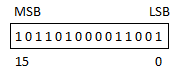
\includegraphics[scale=0.85]{imgs/MSB.png}\end{center}
\section{Umwandlung Hexadezimal und Binär}
Binäre Werte und hexadezimale Werte formen wir direkt um, analog folgender Tabelle:\begin{equation}\begin{tabular}{c | c | c}
Dezimal & Binär & Hexadezimal\\
\hline
0 & 0000 & 0x00\\
1 & 0001 & 0x01\\
2 & 0010 & 0x02\\
3 & 0011 & 0x03\\
4 & 0100 & 0x04\\
5 & 0101 & 0x05\\
6 & 0110 & 0x06\\
7 & 0111 & 0x07\\
8 & 1000 & 0x08\\
9 & 1001 & 0x09\\
10 & 1010 & 0x0A\\
11 & 1011 & 0x0B\\
12 & 1100 & 0x0C\\
13 & 1101 & 0x0D\\
14 & 1110 & 0x0E\\
15 & 1111 & 0x0F\\
\end{tabular}\end{equation}
\section{Negative Zahlen im Binärsystem}
Während wir zur Darstellung von negativen Zahlen im Dezimalsystem die Ziffermenge um das Minus-Symbol erweitern können, ist dies im Binärsystem so nicht möglich. Stattdessen kann das MSB einer binären Zahl das Vorzeichen (engl. "`Sign"') der Zahl bestimmen: 1 steht für negative, 0 für positive Zahlen. Wir nutzen ausserdem das sogenannte Zweierkomplement um die Zahlen umzuwandeln. Das Zweierkomplent wird aus einer beliebigen binären Zahl berechnet, indem man jede Ziffer invertiert und anschliessend 1 dazu addiert:\\
\\
Beispiel: Wir möchten die Zahl $0010_2$ bzw. $2_{10}$ in eine negative Binärzahl verwandeln:
\begin{eqnarray*}
&\mbox{Zweierkomplement(}0010\mbox{)} \\
&= 1101\\
\end{eqnarray*}
Nun addieren wir $1$ zum Resultat:
\begin{eqnarray*}
&& 1101 + 1\\
&=& 1110
\end{eqnarray*}
Wird im Speicher ein Bereich von 4-Bit betrachtet, beispielsweise $1110$, so entsprechen diese Daten je nach Interpretation/Kontext einer anderen Information:\\ \\
Unsigned-Interpretation
\begin{eqnarray*}&&1110 \\
&=& 1 \cdot 2^3 + 1 \cdot 2^2 + 1 \cdot 2^1 + 0 \cdot 2^0 \\
&=& 14_{10} \end{eqnarray*}
Signed-Interpretation
\begin{eqnarray*}&& \mbox{Zweierkomplement(} 1110\mbox{)} = 0010 \\
&=& 0 \cdot 2^3 + 0 \cdot 2^2 + 1 \cdot 2^1 + 0 \cdot 2^0 \\
&=& -2 
\end{eqnarray*}
Weitere Zahlen:
\begin{equation*}\begin{tabular}{c c c}
Unsigned interpretation & & Signed interpretation \\
\hline
0 & 0000 & 0\\
1 & 0001 & 1\\
2 & 0010 & 2\\
3 & 0011 & 3\\
4 & 0100 & 4\\
5 & 0101 & 5\\
6 & 0110 & 6\\
7 & 0111 & 7\\
8 & 1000 & -8\\
9 & 1001 & -7\\
10 & 1010 & -6\\
11 & 1011 & -5\\
12 & 1100 & -4\\
13 & 1101 & -3\\
14 & 1110 & -2\\
15 & 1111 & -1\\ \end{tabular} 
\end{equation*}
Dadurch, dass für das Vorzeichen ein Bit benötigt wird, reduziert sich der Wertebereich (Range) einer Zahl entsprechend:
\begin{eqnarray*}-2^{n-1}, ..., 0, ..., 2^{n-1} - 1 \end{eqnarray*}
Der Wertebereich reicht somit für eine positive Zahl weniger als für negative.
\section{Speichereinheiten}
Die Standard Speichereinheit in einem Computer ist ein Byte. Ein Byte enthält 8 Bit. Diese Zahl ist besonders historisch bedingt. Mit der Entwicklung der Computerarchitekturen, wurden immer grössere Einheiten eingeführt:
\begin{center}
1 byte = 8 bit\\
1 word = 16 bit\\
1 doubleword = 32 bit\\
1 quadword = 64 bit\\
\end{center}
\begin{center}
	\begin{tabular}{l|l|l|l}
			\textbf{Datentyp} & \textbf{Range} & \textbf{Datentyp} & \textbf{Range}\\\hline
			Unsigned byte & $0$ bis $255$ & Signed byte & $-128$ bis $+127$\\\hline
			Unsigned word  & $0$ bis $65'535$ & Signed word & $-32'768$ bis $+32'767$\\\hline
			Unsigned doubleword & $0$ bis $4'294'967'295$ & Signed doubleword & $-2'147'483'648$ bis $+2'147'483'647$\\				
\end{tabular}
\end{center}

\section{Binäraddition}
Wenn zwei binäre Zahlen addiert werden sollen, geschieht dies Bit für Bit, beginnend mit dem LSB. Für die Addition zweier Bits gibt es 4 Möglichkeiten:
	\begin{center}
		\begin{tabular}{l|l}
			$0+0=0$&$0+1 =1$ \\ \hline
			$1+0 = 1$ & $1+1 = 10$ \\
		\end{tabular}
		\end{center}
Der Wert von $1+1=10$ übersteigt offensichtlich den Wertebereich eines Bits und wird Carry (Übertrag) genannt und wird zur Addition der nächsthöheren Stelle mitgenommen. 

Beispiel: $6$ + $10$ = $16$
\begin{center}\begin{tabular}{ccccccc}
& $0$ & $0$ & $0$ & $1$ & $1$ & $0$ \\
+ & $0$ & $0_1$ & $1_1$ & $0_1$ & $1$ & $0$ \\ \hline
& $0$ & $1$ & $0$ & $0$ & $0$ & $0$ \\ \hline \hline
\end{tabular}\end{center}
\subsection{Flags}
Um herauszufinden, ob das angezeigte Resultat einer Rechnung stimmt, setzt der Prozessor sogenannte Flags. 
\\\\
Das \textbf{Carry-Flag} wird gesetzt, wenn das Resultat einer unsigned Rechnung nicht stimmt, d.h. wenn das korrekte Resultat grösser der maximal darstellbaren Zahl ist.\\
\begin{center}
\includegraphics[scale=0.85]{imgs/Carry.png}
\end{center}
Das Carryflag wird auch genutzt, um Additionen grosser Binärzahlen in mehrere Teilschritte aufzuteilen.
\begin{center}
\includegraphics[scale=0.85]{imgs/Carry2.png}
\end{center}
Das \textbf{Overflow-Flag} wird gesetzt, wenn bei einer arithmetischen Operation mit signed-Zahlen das Resultat entweder kleiner der minimal darstellbaren Zahl ist oder grösser der maximal darstellbaren Zahl.\\
\begin{center}
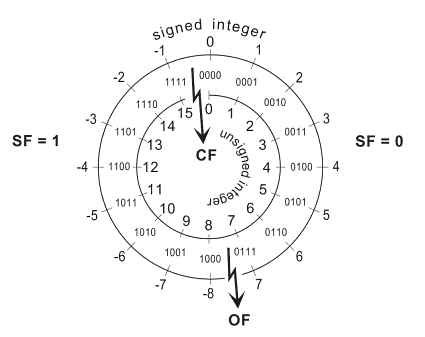
\includegraphics[scale=0.85]{imgs/Zahlenkreis.png}
\end{center}
\noindent Allgemein stellen wir eine Addition wie folgt dar:
\begin{center}\begin{tabular}{ccccccc}
& $a_n$ & $a_{n-1}$ & $...$ & $a_2$ & $a_1$ & $a_0$ \\
+ & $b_n$ & $b_{n-1}$ & $...$ & $b_2$ & $b_1$ & $b_0$ \\ \hline
$c_{n+1}$ & $c_n$ & $c_{n-1}$ & $...$ & $c_2$ & $c_1$ & $c_0$
\end{tabular}\end{center}
Nun finden wir für das Carry-Flag, bzw. das Overflow-Flag folgende Regeln:
\begin{center}
\begin{tabular}{c|c|c|}
& Addition & Subtraktion \\ \hline
Carry-Flag & $C_{n+1}$ & $\lnot C_{n+1}$ \\ \hline
Overflow-Flag & \multicolumn{2}{|c|}{$(a_n \land b_n \land \lnot c_n) \lor (\lnot a_n \land \lnot b_n \land c_n)$} \\ \hline
\end{tabular}
\end{center}
Eine einfach zu merkende Regel für das Overflow-Flag: \\\\
Bei \underline{Signed-Zahlen}: Das Flag wird gesetzt, wenn aus einer Addition zweier positiver Zahlen eine negative folgt oder umgekehrt. \\\\
Bei \underline{Unsigned-Zahlen}: Das Flag wird gesetzt, wenn das Carry des MSB 1 ist.
\\\\
Das \textbf{Sign-Flag} entspricht dem höchstwertigen Bit des Resultats. Es wird zwar immer berechnet, macht jedoch nur bei vorzeichenbehafteten Operanden einen Sinn.\\\\
\begin{center}
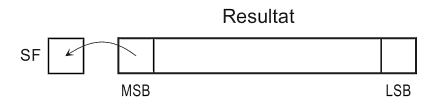
\includegraphics[scale=0.7]{imgs/Sign.png}
\end{center}
Das \textbf{Zero-Flag} zeigt an, ob das Resultat einer Operation null ist. Da die Null bei Zahlen mit und ohne Vorzeichen gleich dargestellt wird, ist keine Unterscheidung nötig. Das Zero-Flag wird aus der invertierten Oder-Verknüpfung (NOR) aller Bits des Resultates gebildet. \\
\begin{center}
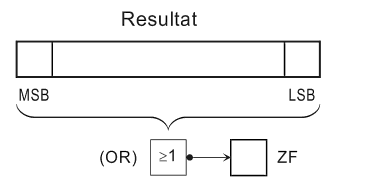
\includegraphics[scale=0.7]{imgs/Zeroflag.PNG}
\end{center}
\section{Zeichenspeicherung}
Man mag sich nun fragen, wie z.B. Buchstaben gespeichert werden können. Dazu werden sogenannte Character Sets benutzt, welche ein Zeichen einer Zahl zuordnen. Bis vor wenigen Jahren wurden dafür nur 8 Bit benutzt. Wegen der grossen Vielfalt an Sprachen wurde dann der 16-Bit Unicode Set eingeführt. \\ \\
Wenn wir im Speicher nun ein Byte mit dem dezimalen Wert 65 finden, so entspricht dieser in Binärschreibweise 01000001. Ein bestimmtes Programm würde dies nun vermutlich in hexadezimaler Schreibweise als 41 ausgeben. Der Grafikkartentreiber hingegen würde stattdessen den Buchstaben A anzeigen, denn 65 entspricht dem ASCII Code für den Buchstaben A.
\newpage\chapter{Digitaltechnik}
\section{Transistoren}
Ein Transistor (kurz für \textbf{trans}fer res\textbf{istor}) ist ein nicht lineares Schaltelement (=Schaltung) und ermöglicht es, mit Strom einen weiteren Strom zu steuern, ohne dass dabei mechanische Bewegungen ausgeführt werden müssen.
\begin{center}
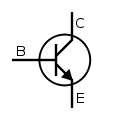
\includegraphics[scale=0.6]{imgs/Transistor.png}
\end{center}
Durch eine kleine Kontrollspannung wird dabei der Stromfluss de- bzw. aktiviert.
\begin{center}
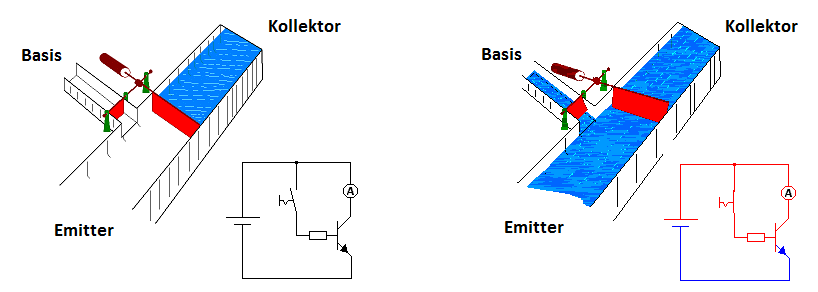
\includegraphics[scale=0.75]{imgs/TransistorFluss.png}
\end{center}
Die Zustände lassen sich mit einer Wahrheitstabelle darstellen:
\begin{center}\begin{tabular}{l|l|l}
a	&	b	& $a \land b$\\ \hline
0	&	0	&	0 \\ \hline
0	&	1	&	0 \\ \hline
1	&	0	&	0 \\ \hline
1	&	1	&	1 \\
\end{tabular}\end{center}
Das \underline{Moorsche Gesetz} besagt, dass sich die Komplexität (= Anzahl Transistoren) integrierter Schaltkreise regelmässig verdoppelt. Je nach Quelle werden 18 oder 24 Monate als Zeitraum genannt. Daraus ergibt sich ein schneller technische Fortschritt. Nach der mechanischen und elektrischen Steuerung von Strömen, fehlt uns heute die Möglichkeit, einen Strom mit Licht steuern zu können. Ein solcher Licht-Transistor würde es ermöglichen, extrem schnelle Supercomputer zu bauen. Die ETH hat in diesem Bereich erste Fortschritte erzielt, allerdings sind diese Transistoren noch weit von einer praktischen Nutzung entfernt.
\section{Logische Gatter}
Unter einem logischen Gatter versteht man ein aus Transistoren realisiertes Element, mit welchem logische Operationen implementiert werden.
\begin{center}\begin{tabular}{c c c c}
Funktion & IEC-Symbol & ANSI-Symbol & Boolsche Formel \\ \hline
AND & 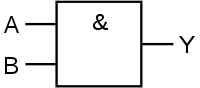
\includegraphics[scale=0.2]{imgs/gatter_IEC_AND.png} & 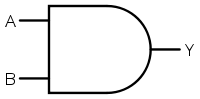
\includegraphics[scale=0.2]{imgs/gatter_ANSI_AND.png} &  $Y = A \land B$ \\
OR & 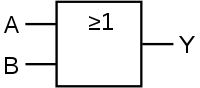
\includegraphics[scale=0.2]{imgs/gatter_IEC_OR.png} & 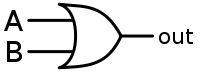
\includegraphics[scale=0.2]{imgs/gatter_ANSI_OR.png} &  $Y = A \lor B$ \\
NOT & 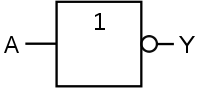
\includegraphics[scale=0.2]{imgs/gatter_IEC_NOT.png} & 
\includegraphics[scale=0.2]{imgs/gatter_ANSI_NOT.png} &  $Y = \lnot A$ \\
NAND & 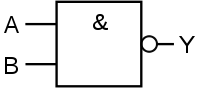
\includegraphics[scale=0.2]{imgs/gatter_IEC_NAND.png} & 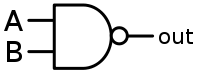
\includegraphics[scale=0.2]{imgs/gatter_ANSI_NAND.png} &  $Y = \lnot (A \land B)$ \\
XOR & 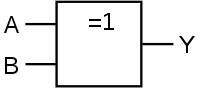
\includegraphics[scale=0.2]{imgs/gatter_IEC_XOR.png} & 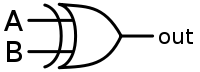
\includegraphics[scale=0.2]{imgs/gatter_ANSI_XOR.png} &  $Y = A \veebar B$
\end{tabular}\end{center}
\section{only-NAND}
Es ist möglich, sämtliche logischen Gatter ausschliesslich mit NAND Gattern zu realisieren. \\ \\
NOT Implementierung mit NAND-Gattern:
\begin{center}
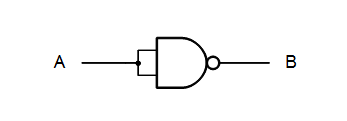
\includegraphics[scale=0.5]{imgs/NAND_NOT.png}
\end{center} 
AND Implementierung mit NAND-Gattern:
\begin{center}
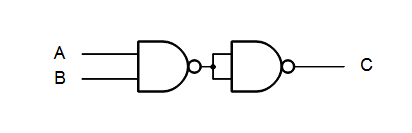
\includegraphics[scale=0.5]{imgs/NAND_AND.png}
\end{center} 
OR Implementierung mit NAND-Gattern:
\begin{center}
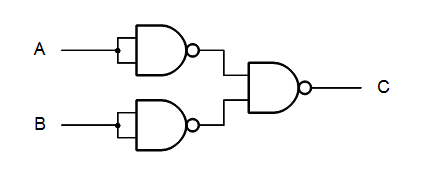
\includegraphics[scale=0.5]{imgs/NAND_OR.png}
\end{center} 
\section{RS-Flipflop}
Ein RS-Flipflop (auch "`Latch"' genannt) ist eine logische Schaltung, mit welcher sich 1 Bit speichern lässt. 
\begin{center}
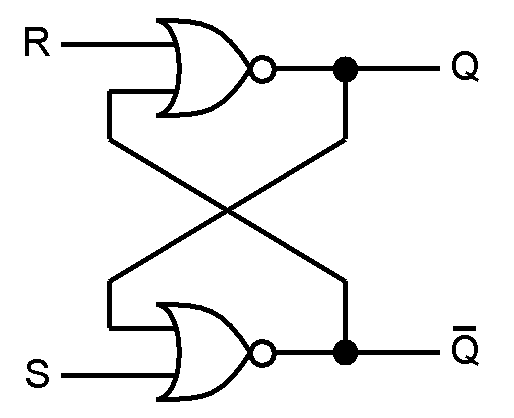
\includegraphics[scale=0.2]{imgs/SRGate.png}
\end{center}
\begin{center}\begin{tabular}{c c | c c}
$S$ & $R$ & Q & $\lnot Q$ \\ \hline
0 & 0 & Q & $\lnot Q$\\
0 & 1 & 0 & 1 \\
1 & 0 & 1 & 0 \\
1 & 1 & - & -\end{tabular}\end{center}
Wenn wir das RS-Flipflop genauer untersuchen, so erkennen wir vier verschiedene Zustände:
\begin{itemize}\item \underline{$S=0$ und $R=0$}: In diesem Zustand zeigen die Ausgänge den gespeicherten Wert des Flipflops an, es gibt keine Veränderung der Ausgangswerte.
\item \underline{$S=1$ und $R=0$}: In diesem Zustand wird das Flipflop, bzw. der Ausgang $Q$ des Flipflops auf 1 gesetzt. Der Ausgang $\lnot Q$ entspreched auf 0.
\item \underline{$S=0$ und $R=1$}: In diesem Zustand wird das Flipflop auf 0 gesetzt. Das bedeutet, dass der Ausgang $Q$ auf 0 gesetzt wird.
\item \underline{$S=1$ und $R=1$}: Illegaler (nicht definierter) Zustand, da es hier eine Race-Condition gibt. \end{itemize}
RS-Flipflops werden beispielsweise bei statischen RAM (SRAM) eingesetzt, da sie sehr schnell sind. Bei einer CPU werden solche Latches beispielsweise für den internen Cache oder die Register eingesetzt.
\section{Multiplexer}
Ein Multiplexer (kurz MUX) ist eine Selektionsschaltung, mit der aus einer Anzahl von Eingangssignalen eines ausgewählt und an den Ausgang durchgeschaltet werden kann. Sie sind vergleichbar mit den früheren Telefonschaltzentralen.
\begin{center}
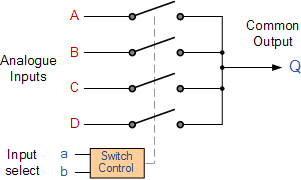
\includegraphics[scale=0.9]{imgs/MUX.png}
\end{center}
\section{Decoder}
\begin{center}
\includegraphics[scale=0.75]{imgs/decoder.png}
\end{center}
\section{Arithmetische Schaltungen}
\subsection{Halbaddierer}
\begin{center}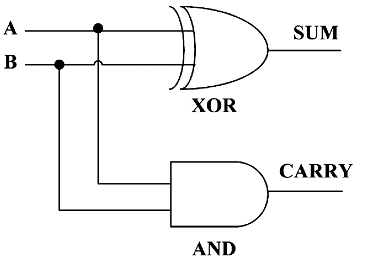
\includegraphics[scale=0.5]{imgs/halfadder.png}\end{center}
Ein Halbaddierer ist eine aus logischen Gattern gebaute logische Schaltung, mit welcher sich zwei Bits addieren lassen. Zusätzlich zum Resultat in Form des Summenbits (0 oder 1) , wird das Carry-Bit ausgegeben, falls die Addition zu einem Übertrag führt. 
\subsection{Volladdierer}
\begin{center}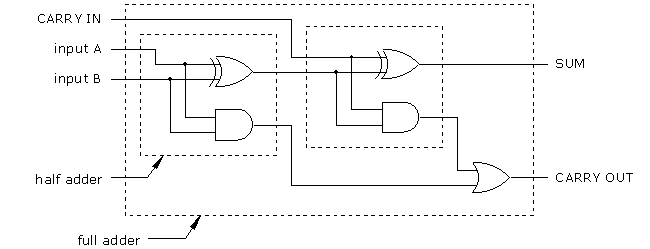
\includegraphics[]{imgs/fulladder.png}\end{center}
Beim Volladdierer handelt es sich um einen Halbaddierer, bei dem zusätzlich das Carry-Bit der vorhergegangenen Addition mitberücksichtigt wird. Zur Implementierung werden meist zwei Halbaddierer verbunden. Mit Volladdierern lassen sich also auch mehrstellige Binärzahlen addieren. Bei der ALU (Arithmetic Logic Unit), einem wichtigten Bestandteil des Prozessors, werden mehrere Volladdierer hintereinander geschaltet, um genau dies zu erreichen.
\subsection{n-Bit Addierer}
Durch Hinternanderreihung mehrerer Volladdierer, können wir auch mehrstellige Bit-Zahlen addieren:
\begin{center}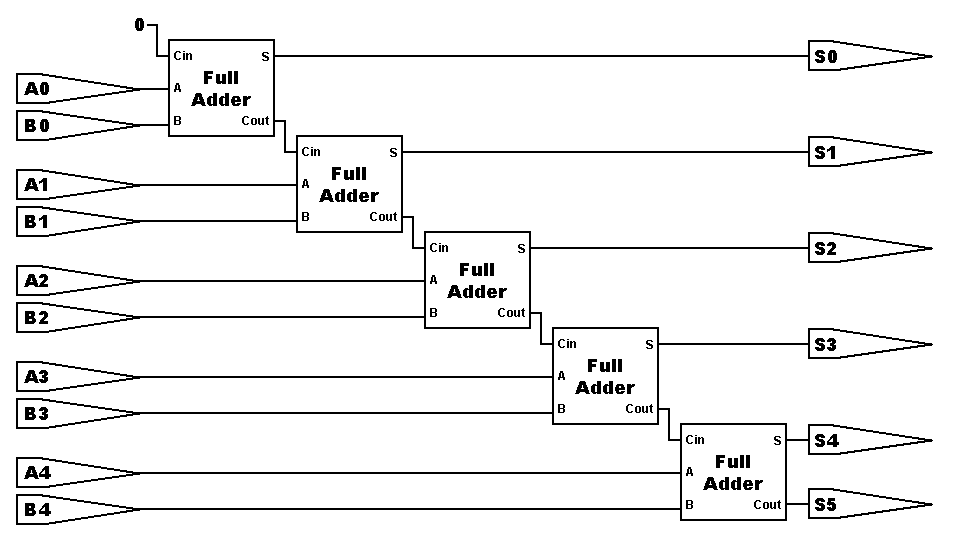
\includegraphics[scale=0.55]{imgs/Ripple.png}\end{center}
\section{Read-only memory}
Read-only memory (ROM) ist ein nicht beschreibbarer Speicher, der aus folgenden Komponenten besteht:
\begin{quote}- Address-Decoder: Durch einen Decoder können mit einer 4-bit Adresse 16 Zeilen angesprochen werden. \end{quote}
\begin{quote}- Memory-Matrix: In jeder der 16 Zeilen stehen 8-Bit zur Speicherung von Werten zur Verfügung.\end{quote}
\begin{center}
\includegraphics[scale=0.85]{imgs/rom.png}
\end{center}
Die vertikale Dimension bzw. die Anzahl Zeilen kann erhöht werden, erfordert dann aber eine Erweiterung des Addressdecoders.
Alternativ kann auch die horizontale Dimension, die Wortbreite, unabhängig davon erhöht werden. Damit können pro Zeile mehr Bits gespeichert werden.
\\ \\
Die einzelnen Bits werden beim ROM durch Sicherungen realisiert, welche bei der Produktion wahlweise durchgebrannt werden, um damit die Werte 0 bzw. 1 zu repräsentieren. Ein nachträgliches Ändern des Speicherinhaltes ist somit nicht möglich. ROMs werden heute nur noch selten eingesetzt und wurden grösstenteils durch PROM (Programmable ROM), EPROM (Erasable Programmable ROM) oder EEPROM (Electrically Erasable Programmable ROM) ersetzt.
\section{Random-access memory}
Im Gegensatz zum ROM, ist der RAM Speicher beschreibbar. RAM besitzt also zusätzlich zu der Memory-Matrix und dem Address-Decoder einen Output Puffer. Mittels eines nWriteEnable Schalters wird bestimmt, ob wir lesen oder schreiben wollen. Mit dem Chipselect Schalter kann der gesamte Chip deaktiviert werden (weder schreiben noch lesen ist mehr möglich).
\begin{center}
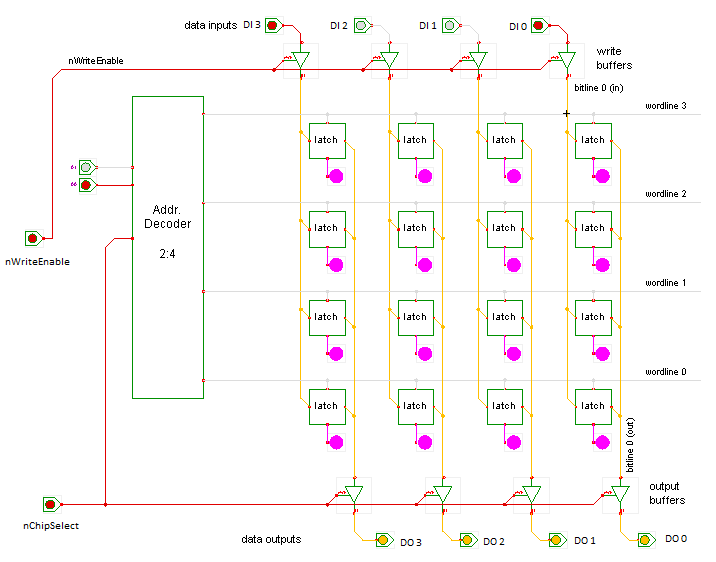
\includegraphics[scale=0.85]{imgs/RAM.png}
\end{center}
Generell können wir bei RAM zwischen zwei verschiedenen Arten unterscheiden: 
\begin{itemize}
	\item \underline{Statisches RAM (SRAM):} Statisches RAM wird mit Transistoren (Latches) realisiert. Dadurch ist SRAM sehr schnell, aber auch sehr teuer und benötigt im Gegensatz zum dynamischen RAM relativ viel Platz.
	\item \underline{Dynamisches RAM (DRAM):} Dynamisches RAM ist mit Kondensatoren aufgebaut. Die Information wird als elektrische ladung im Kondensator gespeichert. Von Vorteil sind hier die tiefen Produktionskosten und die grosse Dichte die erreicht werden kann. Dafür ist DRAM im Vergleich mit SRAM relativ langsam und erfordert einen regelmässigen Refresh der Speicherzellen.
\end{itemize}
\section{Speichergrösse}
Aus der Bezeichnung eines Memorychips kann üblicherweise die Datenmenge bestimmt werden.
Ein 16x8 RAM besitzt 16 Adressen (die mit einem 4 Bit Adressbus und einem 4:16 Decoder angesprochen werden können) und einen Datenbus (Wortlänge) von 8 Bit. Daraus ergibt sich eine Speichergrösse von 128 Bit.\\
Ein 1k x4 RAM hat 1024 Adressen mit je 4 Bit. Um diese 1024 Adresse anzusprechen, wird ein 10 Bit Adressbus benötigt.\\ \\
Einzelne RAM Chips können auf zwei verschiedene Wege miteinander verbunden werden, um die Speichergrösse zu erhöhen:
\begin{enumerate}
	\item Erhöhung der Wortlänge 
	\begin{center}
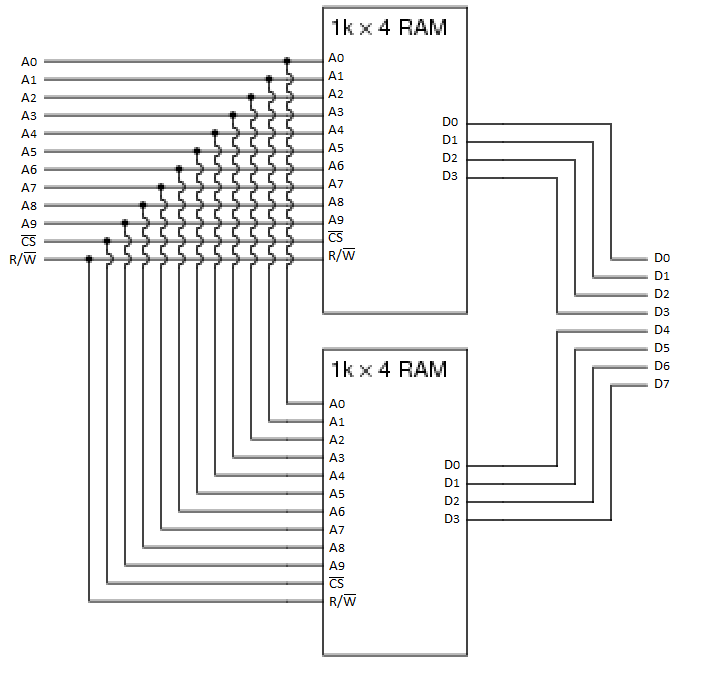
\includegraphics[scale=0.75]{imgs/MemoryArray2.png}
\end{center}
Durch Verdoppelung des Adressbuses, verdoppelt sich die Wortlänge (Die Datenmenge pro Adresse). 
\item Erhöhung der Adressbreite
	\begin{center}
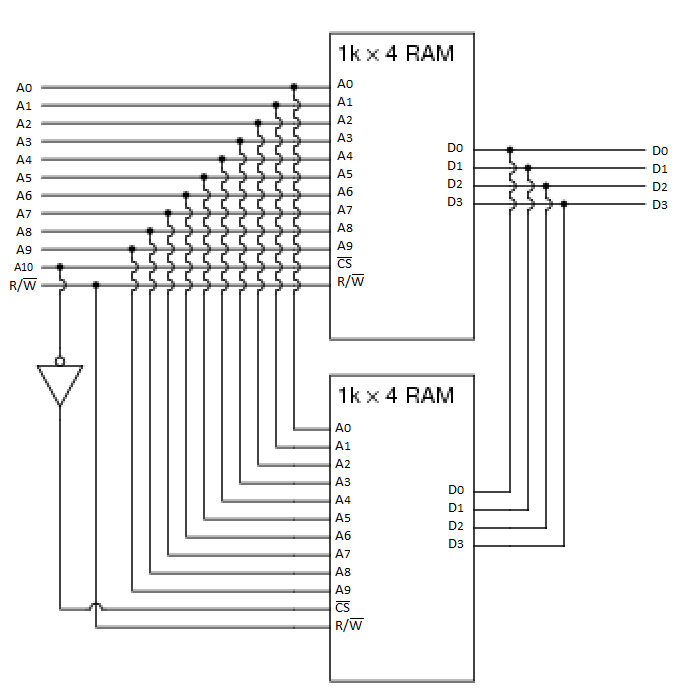
\includegraphics[scale=0.75]{imgs/MemoryArray1.png}
\end{center}
\end{enumerate}
Bei dieser Variante wird der Adressbus verdoppelt, indem ein Bit hinzukommt, welches lediglich den Chipselect beider Memorychips steuert. 
\newpage
\chapter{Computerarchitektur}
\section{Von-Neumann Architektur}
	\begin{center}
		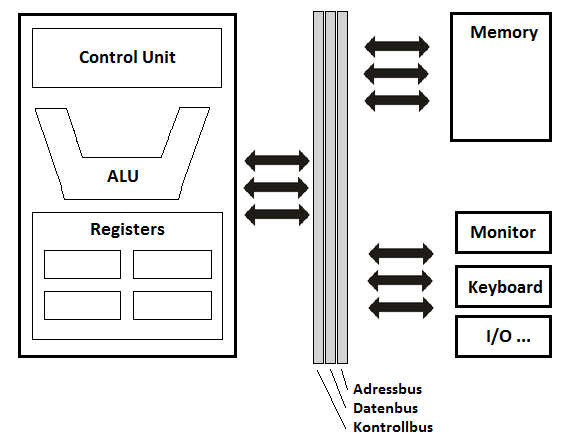
\includegraphics[scale=0.6]{imgs/VonNeumann.png}
	\end{center}
Die Von-Neumann Architektur ist ein Referenzmodell für den Aufbau eines Computers, wonach ein Rechner aus folgenden Komponenten besteht:
\begin{itemize}
	\item CPU - Die zentrale Einheit bestehend aus der ALU, welche Rechenoperationen und logische Verknüpfungen ausführt und der Control Unit, welche die Maschinenbefehle interpretiert und ausführt.
	\item Memory - Speichert sowohl Programme als auch Daten
	\item I/O Units - Steuern Ein- und Ausgabe von Daten zum Anwender (Tastatur, Maus, Bildschirm) und anderen Systemen.
\end{itemize}
\section{CPU}
Die CPU (Central processor unit) besteht aus folgenden Komponenten:
\subsection{ALU (Arithmetic Logic Unit)}
Die ALU führt arithmetische und logische Operationen wie die Addition, die Subtraktion und logische Operationen wie AND, OR und NOT durch. Die ALU ist mit den Registern und über den Datenbus mit dem Memory verbunden. Das Resultat wird an das Ziel-Register bzw. an den Speicher weitergeleitet. Die ALU hält für die Control-Unit einige Flags (Indikatoren) bereit, an denen die CU erkennen kann, wie die Operation verlaufen ist (Überlauf, Gleichheit usw.)
\subsection{CU (Control Unit)}
Die CU koordiniert den Ablauf der Schritte der Befehlsausführung. Sie holt, interpretiert und exekutiert eine Instruktion nach dem anderen. 
\subsection{Clock}
Jede Operation der CPU und des System Bus wird durch die interne Clock synchronisiert, die zu einer konstanten Rate einen Takt vorgibt. Die grundlegendste Zeiteinheit im Computer ist somit ein Machine Cycle.
Die Taktrate der CPU gibt an, wie viele Machine Cycles sie pro Sekunde vorgibt: 1 GHz entspricht 1 Mrd. Cycles pro Sekunde. Ein Machine Cycle dauert somit 1 Nanosekunde. Ein Maschinenbefehl benötigt mindestens einen Cycle, einige jedoch bis zu 50 (z.B. multiply). Befehle, welche Zugriff auf den Arbeitsspeicher verlangen, haben oft leere Cycles (sogenannte Wait states), weil sich die Geschwindigkeit der CPU von der des System Bus und des Speichers unterscheidet.
\section{Register}
Register sind sehr schnelle RAM (SRAM) Bausteine, die bedeutend schneller als das normale Memory benutzt werden können, da sie sich direkt in der CPU befinden.
\subsection{Instruction Pointer (IP)}
Der IP enthält die Speicher-Adresse der Instruktion, die als nächstes zu holen (fetch) und auszuführen (execute) ist. Er wird jeweils nachgeführt (inkrementiert) um soviele Bytes, wie soeben herbeigeschafft wurden. Es ist auch möglich, mit Sprunganweisungen eine komplett andere Speicheradresse zu setzen, die als nächstes zu holen und auszuführen ist.
\subsection{Adress-Register (AR)}
Das AR enthält die Adresse der zu holenden Instruktion oder die Adresse der zu lesenden oder zu schreibenden Daten.
\subsection{Instruktionsregister (IR)}
Das IR enthät in der Fetch Phase die als nächstes auszuführende Instruktion und behält diese bis ans Ende der Ausführung. Das IR hat eine Kapazität, die der längsten aller Instruktionen entspricht. Bei kürzeren Instruktionen werden überzählige Bytes ignoriert.
\subsection{Accumulator / Prozessor Register}
Register wie EAX, BAX etc. werden zur temporären Speicherung von Daten / Adressen genutzt. Sie sind oft Quelle bzw. Ziel von arithmetischen oder logischen Operationen. Der Zugriff ist bedeutend schneller als auf die Daten im Speicher, da sie direkt im CPU Chip implementiert sind, dafür ist deren Anzahl und Speicherplatz beschränkt.
\section{Memory (Programm-/Datenspeicher)}
Der Programm-/Datenspeicher wird zwar oft als Teil des Prozessorsystems betrachtet und ist intensiv daran beteiligt, allerdings ist er nicht Bestandteil der CPU. Sowohl Programme als auch Daten werden im gleichen Baustein gespeichert. Der Programm-Speicher enthält die Programminstruktionen, welche von der CPU fortlaufend geholt und ausgeführt werden. Der Datenspeicher enthält die Plätze für die Variablen, auf welche die Programme zugreifen.
\section{Bussystem}
Die Komponenten sind über ein Bussystem verbunden, welches aus folgenden Komponenten besteht:
\begin{itemize}	
	\item Adressbus - Beinhaltet 8, 16, 32 oder 64 Leitungen (Bit) zur Adressierung des zu lesenden bzw. schreibenden Speichers. Bei einem 32-Bit Datenbus können $2^32$ Speicherzellen (bei 8 Bit pro Zelle entspricht dies ungefähr 4 Gigabyte), die maximal direkt adressiert werden können.
	\item Datenbus - Transportiert Daten zwischen den einzelnen Komponenten. Die Bezeichnung "`32-Bit"' oder "`64 Bit"' CPU bezieht sich üblicherweise auf die Breite des Datenbuses. 	 
	\item Steuerbus - Übernimmt die Kontrolle des Bussystems. Unter anderem wird die Lese-/Schreibsteuerung (Richtung des Databuses) auf dem Steuerbus übertragen.
\end{itemize}
\section{Instruction Set}
Jede CPU besitzt ein sogenanntes Instruction Set - eine Sammlung verschiedener Instruktionen zu deren Programmierung, beispielsweise das Laden eines Wertes aus dem Speicher in ein Register oder das Addieren zweier Zahlen. Da der Prozessor jedoch nur die 0 und die 1 versteht, müssten Programmierer die CPU theoretisch durch sinnvolle Zeichenfolgen wie $10101001 11111111$ programmieren. Damit die Programmierer stattdessen mit symbolischen Bezeichnungen arbeiten können, hat die Control Unit Zugriff auf eine "`Zuordnungstabelle"', in welcher z.B. dem Code $10101001$ bzw. seiner hexadezimalen Entsprechung (Opcode) $A9$ ein sogenannter Mnemonic Code zugeordnet, hier beispielsweise LDA, welcher die CPU zum Laden eines Wertes anweist.\\ \\
\begin{tabularx}{\textwidth}{l|l|l|l}
\textbf{Abstrakt} & \textbf{Mnemonic} & \textbf{Opcode} & \textbf{Maschinencode} \\\hline
Laden des Wertes 255 in ein Register & LDA \#\$FF & A9 FF & 10101001 11111111\\
\end{tabularx}
\section{Instruction Execution Cycle}
Ein Maschinencode Befehl kann in verschiedene Unter-Operationen unterteilt werden, sogenannte Instruction Execution Cycles. Wenn die CPU z.B. eine Operation zweier Zahlen im Speicher durchführen soll, muss sie zuerst die Adresse der beiden Zahlen/Operanden berechnen, die Adressen auf den Addressbus legen, auf den Speicher warten und so weiter. \\ \\
Eine Addition kann in einer Hochsprache wie C/C++ mit einer einzigen, atomaren Instruktion in der Form \textbf{a + b} durchgeführt werden. Ein sogenannter Compiler übersetzt solche Befehle in für den Prozessor verständliche Maschineninstruktionen. Für die genannte Addition sieht dies beispielsweise so ähnlich aus:
\begin{center}
mov Reg $\leftarrow$ [a]\\
add Reg $\leftarrow$ [b]\\
mov [c] $\leftarrow$ Reg\\
\end{center}
Die Schreibweise ist  sehr allgemein gehalten und syntaktisch nicht ganz korrekt. Der Begriff "`Reg"' müsste durch ein in der jeweiligen CPU Architektur existierendes Register (z.B. eax bei Intel Prozessoren) ersetzt werden. Der Pfeil ist ausserdem durch ein Komma zu ersetzen. \\ \\
Bei der Ausführung einer Anwendung wird der Code in den Arbeitspeicher geladen. Anschliessend wir das \textbf{Instruction Pointer Register} (Befehlszähler, Programmcounter). auf die Instruktion des Programmes gesetzt, die als erstes auszuführen ist.  \\ \\
Unter Anweisungen der Control Unit, werden nun folgende Schritte ausgeführt:
\begin{enumerate}
	\item Fetch-Instruction/Phase:
	\begin{itemize}
		\item	Der Inhalt des Instructionpointers wird in das Adressregister übertragen. 
		\item Über das Bussystem wird der Wert dieser Adresse (die Instruktion \textbf{mov eax,[a]} "`gefetched"', d.h., aus dem Speicher gelesen und ins Instruktionsregister geschrieben.
		\item Als nächstes wird der Instructionpointer um so viele Bytes inkrementiert, wie die Instruktion besitzt; er zeigt nun auf die nächste Instruktion.
	\end{itemize}
 \item Decode-Instruction/Phase (Oft als Bestandteil der Fetch-Phase aufgeführt)
  \begin{itemize}	
		\item Die Control-Unit analysiert den erhaltenen Befehl.
	\end{itemize}
	\item Execute-Phase:
	\begin{itemize}	
		\item Die Control-Unit verlangt, dass wir zuerst den Inhalt der Variable a im Speicher auslesen müssen. Dafür wird die Adresse von a ins Adressregister gelegt (die vorhandene wird dabei überschrieben). 
		\item Die adressierte Speicherstelle [a] wird nun ausgelesen und in das angegebene Register gelegt. Die eckigen Klammern zeigen dabei, dass nicht als Konstante, sondern als Speicheradresse zu interpretieren ist. Es wird also der Wert an der Speicheradresse von a gelesen.
		\item Der Inhalt des Programmzählers wird wieder ins Adressregister übertragen; die nächste Instruktion wird gelesen: \textbf{add eax,[b]}. Der Instructionpointer wird wieder inkrementiert.
		\item Nach der Interpretation wird der Wert der Speicherstelle b angefordert
		\item Mit dem Befehl add wird die ALU angewiesen, den gerade ausgelesenen Wert von b mit dem angegebenen Register (in welchem wir den Wert von a abgelegt haben) zu addieren. Das Resultat wird wieder in das Register gespeichert, in welchem der Wert a gespeichert war.
		\item Wieder wird die nächste Instruktion aus dem Speicher gelesen und ins Instruktionsregister übertragen: \textbf{mov [c],eax}. Der Instructionpointer wird inkrementiert.
		\item Nach Analyse der CU wird die Adresse der Variable c ins Adress-Register gelegt, der Wert des Registers auf den Datenbus gelegt und mit dem Schreibbefehl auf dem Control bus werden diese Daten (Das Resultat der Rechnung) in die adressierte Speicherstelle c geschrieben.
	\end{itemize}
\end{enumerate}
\newpage\chapter{6502 Assemblersprache}
\section{Die 6502 Architektur}
Der 6502 Microprocessor gehört zu der 8-Bit CPU Kategorie. Er hat lediglich einige wenige interne Register, 64 kb Memory, einen 16-Bit Addressbus und einen 8-Bit Datenbus. Der 6502 funktioniert nach der "`Little Endian"' Bytereihenfolge, das heisst, das Byte mit den niederstwertigen Bits (d. h. die am wenigsten signifikanten Stellen), wird als erstes genannt.
\begin{center}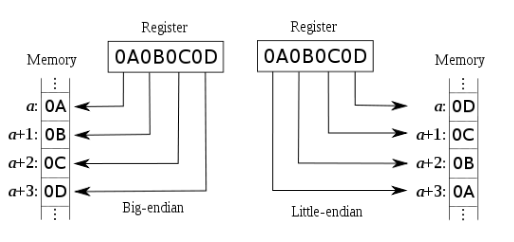
\includegraphics[scale=0.85]{imgs/Endian.png}\end{center}
\subsection{Register des 6502}
\begin{enumerate}
	\item Ein 8-bit Accumulator Register (A)
	\item Zwei 8-bit Index Register (X und Y)
	\item Ein 8-bit Prozessor Status Register (SR)
	\item Ein 8-bit Stack Pointer (SP)
	\item Ein 16-bit Program Counter (PC) bestehnd aus zwei 8-Bit Register PC LowByte (PCL) und PC HighByte (PCH)
\end{enumerate}
\section{Logische / Arithmetische Operationen}
	Logische und arithmetische Operationen werden in der ALU durchgeführt. Sie benötigen jeweils zwei Operanden, die die selbe Grösse haben müssen und aus einem Register, Speicher oder aus einer konstanten Angabe nach dem OP Code stammen.
\begin{center}
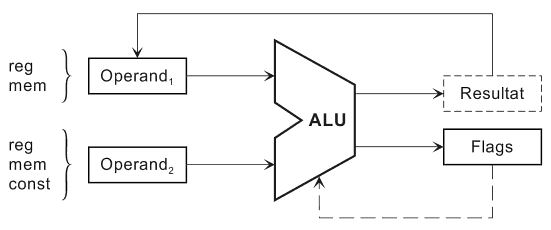
\includegraphics[scale=0.75]{imgs/AsmDatenfluss.png}
\end{center}
\section{Memory Transfers}
Der Grossteil der Maschinen-Instruktionen sind für den Transfer von Daten zwischen dem Speicher und den Registern zuständig. Beispielsweise ermöglicht der Befehl LDA (Load Accumulator) das Laden eines Wertes in das Akku Register (beispielsweise um anschliessend eine Addition oder Subtraktion durchzuführen).
\begin{center}
	\begin{tabularx}{\textwidth}{l|l|X|l}
			\textbf{Addressing Mode} & \textbf{Bsp.} & \textbf{Beschreibung} & \textbf{OP-Code}\\\hline
			Immediate & LDA \#10 & Lädt \$10 (dec. 16) in den Akku & A9 10\\\hline
			Zero Page & LDA \$00 & Lädt den Akku mit dem Wert an der Zero Page Adresse \$00& A5 00\\\hline
			Zero Page,X & LDA \$10,X & Lädt den Akku mit dem Wert an der Zero Page Adresse berechnet aus \$10 addiert mit dem Inhalt des Index Registers X & B5 10 \\\hline
			Absolute & LDA \$1234 & Lädt den Akku mit dem Wert an Adresse \$1234 & AD 34 12\\\hline
			Absolute,X & LDA \$1234,X & Lädt den Akku mit dem Wert an der Adresse berechnet aus \$1234 und dem Wert des Index Registers X & BD 34 12\\\hline
			Absolute,Y & LDA \$1234,Y & Lädt den Akku mit dem Wert an der Adresse berechnet aus \$1234 und dem Wert des Index Registers Y & B9 34 12\\\hline
			(Indirect,X) & LDA (\$20,X) & Lädt den Akku mit dem Wert an der Adresse, welche an der Adresse berechnet aus \$20 addiert mit dem Inhalt des Index Registers X gespeichert ist. & A1 20\\\hline
			(Indirect),Y & LDA (\$20),Y & Lädt den Akku mit dem Wert an der Adresse, berechnet aus dem Wert an Adresse \$20 addiert mit dem Inhalt des Index Registers Y. & B1 20
\end{tabularx}
\end{center}
\section{Addressing Modes}
Grundsätzlich wird zwischen zwei Gruppen von Adressierungsmethoden unterschieden: Den indexierten und den nicht-indexierten. 
\subsection{Accumulator}
Einige Befehle erfordern die Angabe eines Registers, z.B. INC A, oder DEC A
\subsection{Immediate}
Bei einigen Befehlen werden die Daten direkt als zweites Byte nach dem OP-Code angegeben. Dazu wird das Raute Symbol \# genutzt, z.B. \\\\
\begin{lstlisting}[]
LDA #$B2
\end{lstlisting}
Lädt ein Byte (den hexadezimalen Wert B2) in den Akkumulator. Das Symbol \$ zeigt, dass der folgende Wert im Hexadezimalsystem betrachtet wird.
\\\\ 
\begin{tabularx}{\textwidth}{l|l|X}
Fetch/ Execute & Operation & Beschreibung \\ \hline 
Fetch&ABL <- PCL & Programmcounter ins Adr. Register schreiben\\
 &ABH <- PCH & \\
 &R\ $\overline{W}$ <- 1 & Read-mode\\
 &Memory Access & Anweisung ins DBR schreiben\\
 &IR <- DBR & \\ \\
Execute&ABL <- PCL + 1 &  Wert PC + 1 in ABR schreiben\\
 &ABH <- PCH + 1 & \\
 &R\ $\overline{W}$ <- 1 & Read-mode\\
 &Memory Access & Wert ''Erstes Byte'' an Memory[PC+1] lesen\\
 &Akku <- DBR & Wert in Akku schreiben\\
 &PC <- PC + 2 & PC um 2 inkrementieren\\
\end{tabularx}
\subsection{Absolute Addressing}
Bei der absoluten Adressierung wird die Memory Adresse des zu ladenden Wertes direkt angegeben. Diese Adressierungsart ermöglicht somit, die ganzen 65k Bytes des Speichers zu adressieren. \\
Beispiele:\\ \\
Wert an Speicheradresse \$ABCD in den Akku schreiben:\\
\begin{lstlisting}[]
LDA $ABCD
\end{lstlisting}
Der CPU übersetzt LDA zu AD gem. OP Code Liste, die Speicheradresse wird vertauscht. Hexdump:
\\\\
\textbf{AD CD AB}
\\\\
Der Befehl wird nun wie folgt abgearbeitet:\\
\begin{tabularx}{\textwidth}{l|l|X}
Fetch/ Execute & Operation & Beschreibung \\ \hline 
Fetch&ABL <- PCL & Programmcounter ins Adr. Register schreiben\\
 &ABH <- PCH & \\
 &R\ $\overline{W}$ <- 1 & Read-mode\\
 &Memory Access & Nächste Anweisung ins DBR schreiben\\
 &IR <- DBR & Im IR Register steht nun ''AD''\\
 & Instruction == AD & Der CPU erkennt die Funktion AD. Er weiss nun dass die 2 folgenden Bytes die Teile der eigentlichen Adresse sind. Es beginnt der Execute Teil.\\
Execute&ABL <- PCL + 1 &  Wert PC + 1 in ABR schreiben\\
 &ABH <- PCH + 1 &  \\
 &R\ $\overline{W}$ <- 1 & Read-mode\\
 &Memory Access & Wert ''CD'' an Memory[PC+1] lesen\\
 &''Dummy Register'' <- DBR &Ablageort leider nicht bekannt, deshalb nennen wir das Register Dummy Register\\
 &ABH\ L <- PC +2 &  Wert PC + 2 in ABR schreiben\\
 &R\ $\overline{W}$ <- 1 & Auf Read schalten\\
 &Memory Acces &  Wert ''AB'' an Memory[PC+2] lesen\\
 &ABH <- DBR & Wert ''AB'' in ADB High Byte schreiben \\
 &ABL <- ''Dummy Register'' & Wert ''CD'' in ADB Low Byte schreiben\\
 &R\ $\overline{W}$ <- 1 & Auf Read schalten\\
 &Memmory Access & Wert an Speicherstelle \$ABCD lesen\\
 &Akku <- DBR & Wert in Akku schreiben\\
 &PC <- PC + 3 & PC um 3 inkrementieren, ''ADCDAB'' = 3 Byte\\
\end{tabularx}
\subsection{Relative}
Die relative Adressierung wird beim 6502 nur für Branch-Operationen (Verzweigungen) genutzt. Das Byte nach dem OP-Code ist der Verzweigungs-Offset.\\\noindent
Beispiel:\\
Wenn wir Zwei Zahlen vergleichen wollen, können wir den BNE Befehl benutzen. In unserem Beispiel vergleichen wir 6 mit 5. Das Zero Flag bleibt auf 0. BNE lässt den Programmcounter zur Adresse von notequal: jumpen. Diese Adresse ist vom jetzigen Programmcounter aus gesehen, also relativ zur aktuellen Position,  3 Bytes entfernt.\\
\begin{lstlisting}[]
LDA #$06
CMP #$05
BNE notequal
LDA #$09
BRK
notequal:
LDA #$0A
\end{lstlisting}
Im Hexdump wird folgendes ersichtlich.\\
\textbf{d0 03}\\
Der BNE Befehl hat als Paramter 03. Der Programmcounter wird um 3 erhöht und das Programm wird an der Position Programmcounter + 4 fortgesetzt.
\subsection{Zero-Page}
Der Speicher wird beim 6502 mit 16 Bit adressiert und kann somit aufgeteilt werden in zwei 8 Bit (= 2 Byte) Werte, die jeweils 256 Bytes adressieren können. Beim ersten Address-Byte spricht man dabei auch von der Seitenzahl (Pages). Wir haben also insgesamt 256 Pages mit jeweils 256 Adressen. Sämtliche Adressen auf Page 0, also die Adressen \$0000 bis \$00FF können somit mit nur einem Byte angesprochen werden, während das High-Byte immer 0 ist, was der Prozessor bedeutend schneller durchführen kann. Diese Adressen werden auch Zero-Page Adressen genannt. Bsp. LDA \$35 lädt den Wert an der Adresse \$0035 in den Akku. 
\subsection{Indirect}
Diese Adressierung wird nur vom JMP Befehl verwendet. JMP (\$1000) führt dazu, dass der Instruction Pointer auf die Adresse gesetzt wird, die an Adresse 0x1000 gespeichert ist.
\subsection{Absolute Indexed Addressing}
Bei dieser Adressierung wird ein Indexregister (X oder Y) zu einer im 2. und 3. Byte angegebenen absoluten Adresse addiert. Dies ist nützlich, um zum Beispiel 10 Bytes zu füllen, die von der Adresse 0x1009 bis 0x1000 runtergezählt werden.
\subsection{Indexed Zero Page Addressing}
Funktioniert genau wie bei absolute indexed, allerdings ist die Zieladresse auf die ersten 0xFF Bytes limitiert. Falls die Zieladresse über 0xFF rausschaut, wird sie abgeschnitten: LDA \$C0,X und X ist \$60, dann wird die Adresse \$120 (\$C0 + \$60 = \$120) durch abschneiden des Carrys auf \$20 gesetzt.
\subsection{Indexed Indirect Addressing (Indirect,X)}
Bei dieser Adressierung wird der Wert im zweiten Byte zum Wert im X Register hinzuaddiert. Bsp: LDA (\$20,X). Falls X den Wert \$04 enthält, so wird zuerst X zu \$20 addiert (=\$24) und anschliessend der Wert an der Zieladresse aus dem Speicher an Stelle \$24 ins low-Byte und die der Wert an Stelle \$25+1 in das high-Byte geladen, welche zusammen dann die effektive Zieladresse ergeben. Diese muss allerdings in der Zeropage liegen.
\\\\
Beispiel:\\
\begin{lstlisting}[]
LDX #02
LDA ($15, X)
\end{lstlisting}
Speicher:
\\
\\
\begin{tabular}{|c|c|}
\hline
\$0017 &EF  \\ \hline
\$0018 &CD \\ \hline
... &  \\  \hline 
\$CDEF &09  \\ \hline
\end{tabular}
\\
\\
\\
Der Wert 02 im X Register wird zu \$15 addiert. Es ergibt sich die Adresse \$17. \\
Nun werden die Werte an der Adresse \$17 und \$18 ausgelesen. Die Werte sind \$17 = EF und \$18 = CD.
Die neue Adresse ist \$CDEF. Dert Wert 09 von der Adresse \$CDEF wird in den Akku geladen.

\subsection{Indirect Indexed Addressing (Indirect),Y}
Dieser Modus nutzt nur das Y-Register. Das zweite Byte der Instruktion zeigt auf eine Memory Adresse in der Zeropage. Der Inhalt dieser Speicheradresse wird zum Inhalt des Y Registers addiert, das Resultat ist das Low Byte der effektiven Adresse. Der Übertrag dieser Addition wird zum Inhalt der nächsten Zeropage Adresse addiert, was dann das High Byte der effektiven Adresse ergibt. 
\\
Beispiel:
\\\\Speicher:
\\
\\
\begin{tabular}{|c|c|}
\hline
\$0015 &CD  \\ \hline
\$0016 &AB \\ \hline
... &  \\  \hline 
\$ABCF &08  \\ \hline
\end{tabular}
\\\\
Beispiel:\\
\begin{lstlisting}[]
LDY #02
LDA ($15),Y
\end{lstlisting}
Zuerst werden die Werte an der Speicheradresse \$15 und \$16 ausgelesen. Dies ergibt die Adresse \$ABCD. Nun wird der Wert aus dem Y-Register (\$2) hinzuaddiert. Dies ergibt nun die effektive Zieladresse \$ABCF, an welcher der Wert \$08 in den Akku geladen wird.
\section{Conditional Jumps}
Um If-Else Abfragen mit Assembler zu realisieren, werden sogenannte Conditional Jumps benutzt, um in bestimmten Fällen (wenn bestimmte Flags gesetzt sind) an einen neuen Ort im Programm zu springen.
Um die Flags zu setzen, ohne dabei die Register zu überschreiben, gibt es den Befehl CMP, welcher eine Subtraktion des einen mit dem anderen Wert durchführt. Falls das Resultat dieser Subtraktion 0 ist (das Zeroflag wird gesetzt), so stimmen die beiden zu vergleichenden Werte überein. Nun können wir mit dem Befehl BEQ (Branch Equal) zu einer Speicheradresse springen, in welchem dieser Fall abgearbeitet wird. Mit BNE (Branch Not Equals) können wir somit die Else Verzweigung, als den Fall, dass die beiden Werte nicht übereinstimmen, abfangen.

\subsection{Conditional Jump x86 Spezifisch}
\subsubsection{unsigned}
\begin{tabularx}{\textwidth}{l l l l}
Relation&Differenz&Flags&Memonic\\ \hline
A = B & A - B= 0& z & jeq <adr> (equal)\\
$A \not = B$&$A - B \not = 0$& $\overline{z}$&  jne <adr> (notequal)\\  
A < B & A - B < 0 & c & jb <adr> (below)\\
$A \leq B$& $A - B \leq 0$& $c \lor z$ & jbe <adr> (belowequal)\\
 A > B & A - B > 0 &$ \overline{c\lor z}$ & ja <adr> (above)\\
$A \geq B$& $A - B \geq 0$& $ \overline{c\lor z} \lor z$ & jae <adr> (aboveequal)\\
\end{tabularx}
\subsubsection{signed}
\begin{tabularx}{\textwidth}{l l l l}
Relation&Differenz&Flags&Memonic\\ \hline
A = B & A - B= 0& z & jeq <adr> (equal)\\
$A \not = B$&$A - B \not = 0$& $\overline{z}$&  jne <adr> (notequal)\\  
A < B & A - B < 0 & s xor of & jl <adr> (less)\\
$A \leq B$& $A - B \leq 0$& (s xor of)$\lor z $ & jle <adr> (lessequal)\\
 A > B & A - B > 0 &$ \overline{(s xor of)\lor z }$ & jg <adr> (greater)\\
$A \geq B$& $A - B \geq 0$& $ \overline{s xor of}$ & jge <adr> (greaterequal)\\
\end{tabularx}
\section{Stack}
Der Stack ist ein spezieller Bereich des Memory. Den Stack kann man sich wie ein Stapel Bücher vorstellen, auf welchen man die Bücher eines nach dem anderen stappelt und später, beim zuletzt hingelegten Buch, anfängt wieder zu entfernen (auch LIFO "`Last in, first out"'-Prinzip genannt).

\begin{center}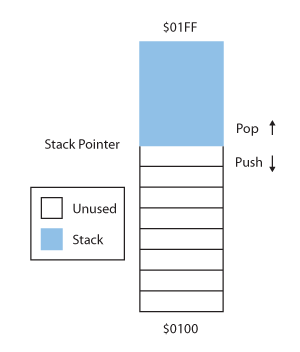
\includegraphics[scale=0.8]{imgs/stack.png}\end{center}

Wird in Hochsprachen wie C, C++ oder Java in einer Funktion eine lokale Variable erstellt, so wird diese im Stack gespeichert. In Assembler gibt es diverse Instruktionen, die mit dem Stack arbeiten.
\subsection{PHA: Push Akku Value on Stack}
Unser Beispiel: \\
\\
Code:\\
\textbf{PHA}
\\
Wert des Akkus wird auf den Stack gelegt\\
\\
\\
\begin{tabularx}{\textwidth}{l|l|X}
Fetch/ Execute & Operation & Beschreibung \\ \hline 
Fetch& ABL <- PCL& PC in Adressbusregister schreiben\\
& ABH <- PCH& \\
&R\ $\overline{W}$ <- 1& Auf Read schalten\\
&Memory Acces& Nächste Anweisung lesen\\
&IR <- DBR& Anweisung in IR Register schreiben\\
&IR = 48 & Der CPU erkennt die Funktion 48. Es beginnt der Execute Teil.\\
Execute&ABL <- SP& Stackpointer Wert in AB Low Byte schreiben\\
&ABH <- 0x01& Wert 0x01 in AB High Byte schreiben, Standard bei Stackpoint\\
&DBR <- A& Wert des Akkumulators in DBR schreiben\\
&R\ $\overline{W}$ <- 0& Auf Write schalten\\
&Memory Access&  Wert des Akkus auf Stack legen\\
&SP <- SP -1& Stackpointer dekrementieren\\
&PC <- PC + 1& PC um 1 erhöhen\\
\end{tabularx}

\subsection{PHP: Push Programcounter Value on Stack}
Unser Beispiel: \\
\\
Code:\\
\textbf{PHP}
\\
Wert des Programmcounters wird auf den Stack gelegt\\
\\
\\
\begin{tabularx}{\textwidth}{l|l|X}
Fetch/ Execute & Operation & Beschreibung \\ \hline 
Fetch& ABL <- PCL& PC in Adressbusregister schreiben\\
& ABH <- PCH& \\
&R\ $\overline{W}$ <- 1& Auf Read schalten\\
&Memory Acces& Nächste Anweisung lesen\\
&IR <- DBR& Anweisung in IR Register schreiben\\
&IR = 08 & Der CPU erkennt die Funktion 08. Es beginnt der Execute Teil.\\
Execute&ABL <- SP& Stackpointer Wert in AB Low Byte schreiben\\
&ABH <- 0x01& Wert 0x01 in AB High Byte schreiben, Standard bei Stackpoint\\
&DBR <- PC& Wert des Programcounters in DBR schreiben\\
&R\ $\overline{W}$ <- 0& Auf Write schalten\\
&Memory Access&  Wert des Akkus auf Stack legen\\
&SP <- SP -1& Stackpointer dekrementieren\\
&PC <- PC + 1& PC um 1 erhöhen\\
\end{tabularx}

\subsection{PLA: Pop Data from Stack, store it in Akku}
Unser Beispiel: \\
\\
Code:
\\
\textbf{PLA}
\\
''Oberster'' Wert der auf dem Stack wird in den Akku geschrieben.\\
\\
\\
\begin{tabularx}{\textwidth}{l|l|X}
Fetch/ Execute & Operation & Beschreibung \\ \hline 
Fetch& ABR <- PC &  PC in Adressbusregister schreiben\\
&R\ $\overline{W}$ <- 1& Auf Read schalten\\
&Memmory Access& ZUgriff auf Memory, nächste Anweisung lesen\\
&IR <- DBR&\\
&IR = 68& Der CPU weiss, nun muss er einen PLA Befehl abarbeiten \\
Execute&ABL <- SP+1& Stackpointer + 1 in ABL schreiben\\
A <- Mem[SP+1]&ABH <- 0x01& ABH auf 0x01 setzen, Standard bei Stack\\
&R\ $\overline{W}$ <- 1& Auf Read schalten\\
&Memory Acces& Lesen n Speicherzelle Mem[SP+1]\\
&A <- DBR& Wert in Akku schreiben\\
&SP <- SP+1& Stackpointer um 1 inkrementieren\\
&PC <- PC + 1& PC um 1 inkrementieren\\
\end{tabularx}

\subsection{Endian}
\begin{tabularx}{\columnwidth}{X|X}
Little Endian & Big Endian\\ \hline
Bei Little-Endian (wörtlich „Klein-Ender“) wird das Byte mit den niederstwertigen Bits (Rechts) an der kleinsten Speicheradresse gespeichert &Bei Big-Endian (wörtlich „Groß-Ender“) wird das Byte mit den höchstwertigen Bits (Links) zuerst gespeichert, das heißt an der kleinsten Speicheradresse
\end{tabularx}
\begin{myexample}
Im folgenden Beispiel wird die Ganzzahl 439.041.101 (Vierhundertneununddreißig Millionen...) als 32-Bit-Integer-Wert gespeichert (Binär: 00011010 00101011 00111100 01001101, hexadezimal: 1A 2B 3C 4D). Die Speicherung erfolgt in vier Bytes ab der hypothetischen Speicheradresse 10000.
\begin{center}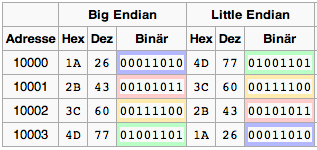
\includegraphics[scale=0.6]{imgs/endians.png}\end{center}
\end{myexample}
\newpage
\section{Subroutines}
Sub\underline{routine}n ermöglichen, oft benutzte Codeprozeduren auszulagern und aufrufen zu können. Zu einer Subroutine gehört beispielsweise deren Bezeichnung, Übergabewerte (Parameter) um dynamischen Einfluss auf deren Funktion zu haben und der Rückgabewert. Funktionen mit Hilfe eines speziellen Bereichs im RAM ermöglicht, dem Stack. Um in eine Subroutine zu springen, nutzen wir den Befehl JSR (Jump to Subroutine).\\
Wollen wir von der Subroutine zum normalen Programmfluss zurückkehren, nutzen wir die RTS (Return from Subroutine).
\subsection{JSR}
Der JSR Befehl hat 2 Aufgaben
	\begin{itemize}
		\item Aktueller PC + 2 auf Stack legen. Dient als Returnadresse für den RTS Befehl\\
			ST <- PCL\\
			ST+1 <- PCH
		\item
			Zur Angegebenen Adresse jumpen
	\end{itemize}
\subsection{RTS}
Mit dem RTS Befehl springen wir von aus einer Subroutine zurück in den normalen Programmfluss.
Als Zieladresse dient hier der PC, der während dem JSR Befehl auf den Stack gelegt wurde.\\
Diese Adresse wird vom Stack gepopt und in den PC geschrieben.
\newpage
\chapter{Die Programmiersprache C}
C ist eine Hochsprache, das heisst, sie abstrahiert die Assemblersprachen. Trotzdem ist C sehr systemnahe, weshalb Betriebssysteme normalerweise in C geschrieben werden. Während Assembler quasi 1 zu 1 in den Bytecode der Maschinenbefehle umgewandelt wird, ist C Code für die CPU unverständlich und muss zuerst mit Hilfe eines Compilers in die Assemblersprache der jeweiligen CPU übersetzt werden.
\section{Variablen}Der Compiler/Linker reserviert im Speicher eine bestimmte Anzahl Bytes in Form eines zusammenhängenden Blocks, welchem ein Namen zugeordnet wird, über welchen der Programmierer zugreifen und mit einem Wert versehen kann. Die Grösse dieses Speicherblocks und der Interpretationskontext wird durch einen Datentyp definiert. Für ganze Zahlen gibt es beispielsweise den Typ "`Integer"', welcher auf den meisten Computern 4-Byte an Speicher benötigt.\\\\ Beispiel: Mit
\begin{lstlisting}[]
int x = 1;
\end{lstlisting}
können wir eine Variable vom Typ Integer definieren. Es werden 4-Byte im Speicher reserviert, auf die wir fortan über den Namen i zugreifen können. 
\begin{center}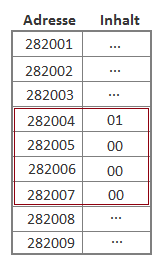
\includegraphics[scale=0.85]{imgs/c-variablen.png}\end{center}
\section{Pointers}
Ein Pointer ist eine Variable, die als Wert eine Speicheradresse besitzt und somit auf eine andere Variable "`zeigt"'. 
\subsection{Einfaches Dereferenzieren}
Beispiel:\\
\begin{lstlisting}[]
char value = 'c';
char *p = &value;
\end{lstlisting}
Zeile 1 erzeugt eine Variable namens "`value"', die ein einzelnes Zeichen (Char) speichert und sich bsw. an Adresse 8000 befindet. In Zeile 2 definieren wir mit Hilfe des *-Zeichens einen Pointer vom Typ char, welchem wir mit dem Referenzoperator (\&) die Adresse der Variable "`value"' zuordnen.\\ \\
Um nun auf den Wert zuzugreifen, auf den unser Pointer p2 zeigt, nutzen wir den Dereferenzierungsoperator (*):\\
\begin{lstlisting}[]
*p    // Wert des Ziels des Pointers p: 'c'
p 		// Wert des Pointers p: 0x8000
&p 		// Adresse des Pointers p: 0x5000
\end{lstlisting}
\begin{center}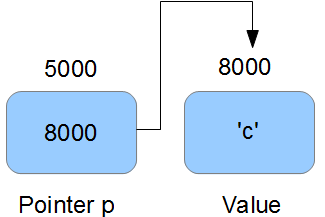
\includegraphics[scale=0.6]{imgs/c-pointers.png}\end{center}

\subsubsection{Weitere Beispiele:}

Deferenzieren vom Pointer ermöglicht uns auf i zuzugreifen. *ip leitet uns zur Variable  i weiter.
\begin{lstlisting}[frame=single] 
int i;
/* Define a Pointer for Variable i */
int *ip;
i = 5;
/* Set ip Value to Adress of i */
ip = &i;
/* Dereference of  *ip = Acces to Variable i/ Systemaddress of i, 
set value of i */
*ip = 7;
\end{lstlisting}
\bigskip
Der Pointer jp soll nun auf i zeigen. Wie kann das realisiert werden?
\begin{lstlisting}[frame=single] 
int j,
int *jp,
int i,
int ip,
ip = &i;

/* Solution */
jp = ip
\end{lstlisting}
Wir haben zwei Variabeln und wollen deren Wert tauschen /swappen.
\begin{lstlisting}[frame=single] 
int a = 5;
int b = 7;
/* Target a = 7, b = 5 */

/*Solution:
We define a function for swapping, we use pointers as parameter*/
swap(int *ap, int *bp)
{
	int dummy = *ap;
	*ap = *bp;
	*bp = dummy;
}

/* We call the function this way */
swap(&a,&b);
\end{lstlisting}
\newpage

\subsection{Doppeltes Dereferenzieren}
Es ist ausserdem möglich, Zeiger auf Zeiger zu erstellen.\\
Doppeltes Auflösen des Pointers. Pointer beinhaltet Pointer.\\
\begin{lstlisting}[]
char value = 'c';
char *p = &value;
char **p2 = &p;
\end{lstlisting}
\begin{center}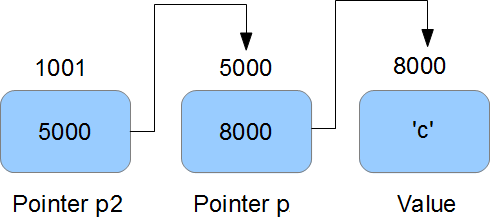
\includegraphics[scale=0.6]{imgs/c-pointers2.png}\end{center}
\begin{lstlisting}[]
*p2 		// Wert auf den p2 zeigt: Die Speicheradresse 8000
**p2 		// Wert auf den p1 zeigt, auf welchen p2 zeigt: 'c'
p2 			// Wert des Pointers p2: Die Speicheradresse 5000
&p 			// Adresse des Pointers p: Die Speicheradresse 1001
\end{lstlisting}

\subsubsection{weiteres Beispiel}

\begin{lstlisting}[frame=single] 
int i;
int *ip;
ip = &i;
/* Define a double Pointer */
int **ipp;
/* Set ipp value to Address of ip */
ipp = &ip;
/* Set value of i = 9 */
**ipp = 9;
/* **ipp -> *ip -> i/
\end{lstlisting}
\newpage

\section{Nutzen von Pointern}
In C geschieht die Werteübergabe an Subroutinen standardmässig nach dem "`\textbf{Call By Value}"' Prinzip. Es gibt in C (erst in C++) kein "`\textbf{Call By Reference}"' wie in anderen Sprachen. Bsp: \\
\begin{lstlisting}[]
void doubleValueOf(int i){
		i = 2*i;
}

void main(){
		int zahl = 5;
		doubleValueOf(zahl);
}
\end{lstlisting}
Wenn wir die Funktion "`doubleValueOf"' aufrufen, wird der Wert der Variable "`\textit{zahl}"', auf den Stack gelegt und innerhalb der Funktion darauf zugegriffen. Die ursprüngliche Variable "`\textit{zahl}"' liegt jedoch an einer Stelle im Speicher, die der Funktion nicht bekannt ist. Es wird somit der Wert einer Kopie der Variable "`\textit{zahl}"' verdoppelt, die nach Ende der Funktion verloren geht. Zurück in unserem Hauptprogramm, wird die Variable "`\textit{zahl}"' immer noch 5 als Wert haben. \\\\
Pointer ermöglichen nun, statt einer Kopie einen Referenz auf die richtige Variable "`zahl"' zu übergeben.\\
\begin{lstlisting}[]
void doubleValueOf(int *pi){
		*pi = 2*(*pi); // Der Wert der Adresse, auf die pi zeigt, wird auf 2* den Wert von i (*i) gesetzt.
}

void main(){
		int zahl = 5;
		doubleValueOf(&zahl);
}
\end{lstlisting}
\section{Arrays}
Arrays sind Felder/Reihungen von Variablen eines bestimmten Datentypes. Beispiel:\\
\begin{lstlisting}[]
int ar[5] = {1, 2, 3, 4, 5}
\end{lstlisting}
Erstellt 5 aufeinanderfolgende Integer Variablen mit den Werten 1,2,3,4 und 5. Wir können direkt auf ein bestimmten Element zugreifen:\\
\begin{lstlisting}[]
ar[2] = 7;
\end{lstlisting}
Wenn ein Integer 4 Byte beansprucht, ist die Grösse des gesamten Arrays $5 \cdot 4$ Byte = 20 Byte. \\\\
C besitzt standardmässig keinen Datentyp "`String"', um Zeichenfolgen darzustellen. Stattdessen können wir ein Array von Chars benutzen:\\
\begin{lstlisting}[]
char str[6] = {'H','a','l','l','o','\0'};
\end{lstlisting}
Das Zeichen '\textbackslash 0' wird benötigt, um das Ende eines Strings zu markieren. Wir können auch \\
\begin{lstlisting}[]
char str[] = "Hallo";
\end{lstlisting}
schreiben. Dies erstellt ein Array mit 6 Char Elementen, 5 für "`Hallo"' und ein weiteres für '\textbackslash 0'.
Eine weitere Möglichkeit wäre es, einen Zeiger auf ein Char Array zu erstellen:\\
\begin{lstlisting}[]
char *str = "Hallo";
\end{lstlisting}
Dabei wird sowohl ein (verstecktes) Char Array mit dem Inhalt \{'H','a','l','l','o'\} und einen Char Pointer namens str erstellt, der auf das erste Element des versteckten Arrays zeigt. str zeigt nun also auf das erste Char-Element, den Buchstaben 'H':\\
\begin{lstlisting}[]
*str 				// 'H', oder auch str[0]
*(str+1) 		// 'a', oder auch str[1]
*(str+5) 		// 'a'
\end{lstlisting}
Achtung: Es ist undefiniert was passiert, wenn nun *str ein neuer Wert zugeordnet wird!

\section{Dynamische Speicherallozierung/ Dynamic Memory Allocation}
Lokale und globale Variablen werden normalerweise statisch, d.h. beim Starten des Programms reserviert. Manchmal ist es notwendig, Speicher dynamisch, zur Laufzeit, anzufordern, beispielsweise weil man auf Benutzereingaben reagieren will oder weil man eine Variable einer bestimmten Grösse benötigt. \\ \\
Die Programmiersprache C bietet dafür einige Funktionen zur Verfügung.
\begin{mydef}
	Statisch bedeutet, dass der benötige Speicher zu beginn des Programms reserviert wird.
\end{mydef}
Ein Beispiel:
\begin{lstlisting}[frame=single] 
int a;
int *ip;
int array[10];
\end{lstlisting}
\begin{mydef}
	Dynamisch bedeutet, dass der benötige Speicher zur Laufzeit des Programms reserviert wird.
\end{mydef}
Um den Speicher zur Laufzeit zu reservieren schreiben wir:
\begin{lstlisting}[frame=single] 
int *ip;
ip = malloc(sizeof(int)*10);
\end{lstlisting}
Damit reserviren wir den Platz für 10 int Werte, also ein Array der Grösse 10.
Ein int ist 32Bit gross, dementsprechend werden 320Bit oder 40Byte reserviert.\\
\\
Der Befehl malloc (Memory allocation) gibt die Speicheradresse des ersten int Blocks zurück. Wir speichern diesen in einem Pointer.\\
\\
Aufgabe:\\
Wert 3 an erste Speicheradresse im Array schreiben
\begin{lstlisting}[frame=single] 
*ip = 3;
\end{lstlisting}
*ip wird dereferenziert wir erhalten Zurgiff zur ersten Speicheradresse\\
\\
Aufgabe2:\\
Wert 2 an zweite Speicheradresse im Array schreiben
\begin{lstlisting}[frame=single] 
*(ip+1) = 2;
\end{lstlisting}
Dadurch dass wir int *ip schreiben, weiss der Compiler wie weit er mit *ip+1 springen muss. Da es sich um int Werte handelt, rechnet er zur ersten Speicheradresse 4 Byte hinzu. *ip+2 rechnet er 8Byte hinzu. usw.\\
\\
Achtung!
\begin{lstlisting}[frame=single] 
*(ip+100) = 1
\end{lstlisting}
Ist nicht möglich, schliesslich haben wir nur 10 int Blöcke reserviert. Die Adresse liegt ausserhalb des Speicherbreichs.

\newpage
\section{Speichersegmente}
\begin{tabular}{l l}
RAM & Programm 1 \\
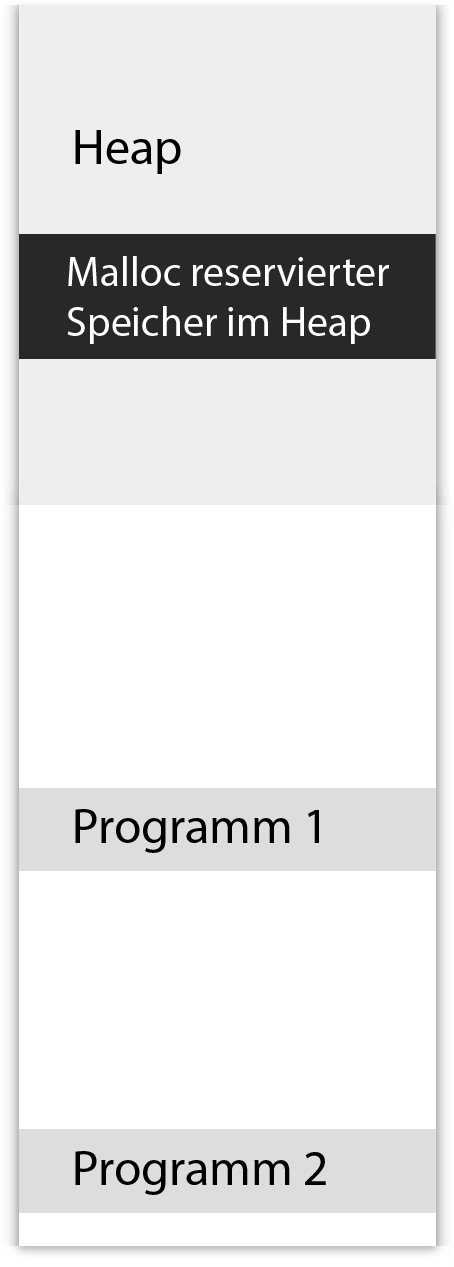
\includegraphics[]{imgs/ram_segments.png}&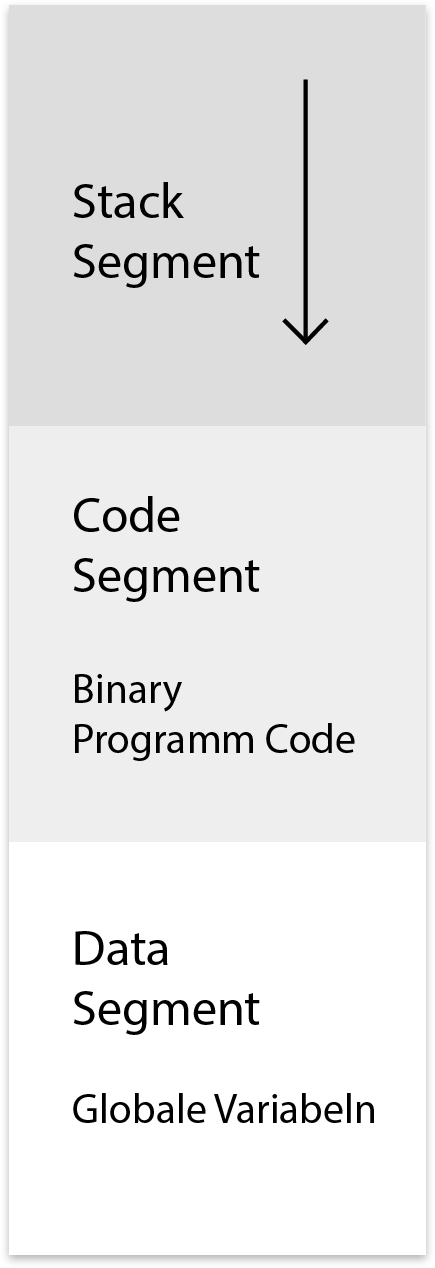
\includegraphics[]{imgs/prg_segments.png}\\
Der Heap Bereich ist der freie Speicher& \\
\end{tabular}

\newpage
\section{Listen}
Eine unbekannte Anzahl Elemente verwalten.
\begin{lstlisting}[frame=single] 
struct element
{
	int data; // The Data of the element
	struct element *next; // the next element
}
\end{lstlisting}
Wir definieren das ''Objekt'' element, es besitzt einen Wert und einen Pointer auf das nächste element Objekt.

Um eine Verlinkte Liste von Elementen mit den werten 1,2,3... zu erstellen, gehen wir wie folgt vor:
\begin{lstlisting}[frame=single] 
struct element
{
	int data; // The Data of the element
	struct element *next; // the next element
}

struct element *head;
struct element *np; // next Pointer

/* 1 */
// reservate space for the first element
head = malloc(sizeof (struct element));

/* 2*/
(*head.data) = 1; // Set data 

/* 3 */
// reservate space for the next Element
np = malloc(sizeof(struct node));

/* 4 */
(*head).next = np;

/* 5 */
// Set data
(*((*head).next)).data = 2;

/* 6 */
// Shorter Version
np->next = malloc(sizeof(struct node));
np->next->data = 3;
\end{lstlisting}
\newpage
Kurze Version:
\begin{lstlisting}[frame=single] 
struct element
{
	int data; // The Data of the element
	struct element *next; // the next element
}
struct element *np; // next Element Pointer

/* 1. Element */
np = malloc(sizeof(struct element));
np->data = 1;
np->next = malloc(sizeof(struct element));

/* 2. Element */
np = np->next;
np->data = 2;
np->next = malloc(sizeof(struct element));

//... 
\end{lstlisting}
\newpage
\section{Operator Precedence}

\subsection{Beispiele}
\begin{tabularx}{\textwidth}{l|X}
 \textbf{C-Code}& \textbf{Aussage}\\ [2ex] \hline 
int *x(char)&x as function (char) returning pointer to int\\ [2ex]\hline
int (*x)(char)&x as pointer to function (char) returning int\\[2ex] \hline
int *(*x[5])&dx as array 5 of pointer to pointer to int \\[2ex] \hline
int *x(int, char *)& x as function (int, pointer to char) returning pointer to int\\ [2ex] \hline
int *(*x)(int, char *)&x as pointer to function (int, pointer to char) returning pointer to int\\ [2ex] \hline
int (**x)(int, char *)& x as pointer to pointer to function (int, pointer to char) returning int\\ [2ex] \hline
int **x(int *)&declare x as function (pointer to int) returning pointer to pointer to int\\ [2ex] \hline
int (*x[5])(int) &declare x as array 5 of pointer to function (int) returning int \\ [2ex] 
\end{tabularx}


\chapter{Tables}
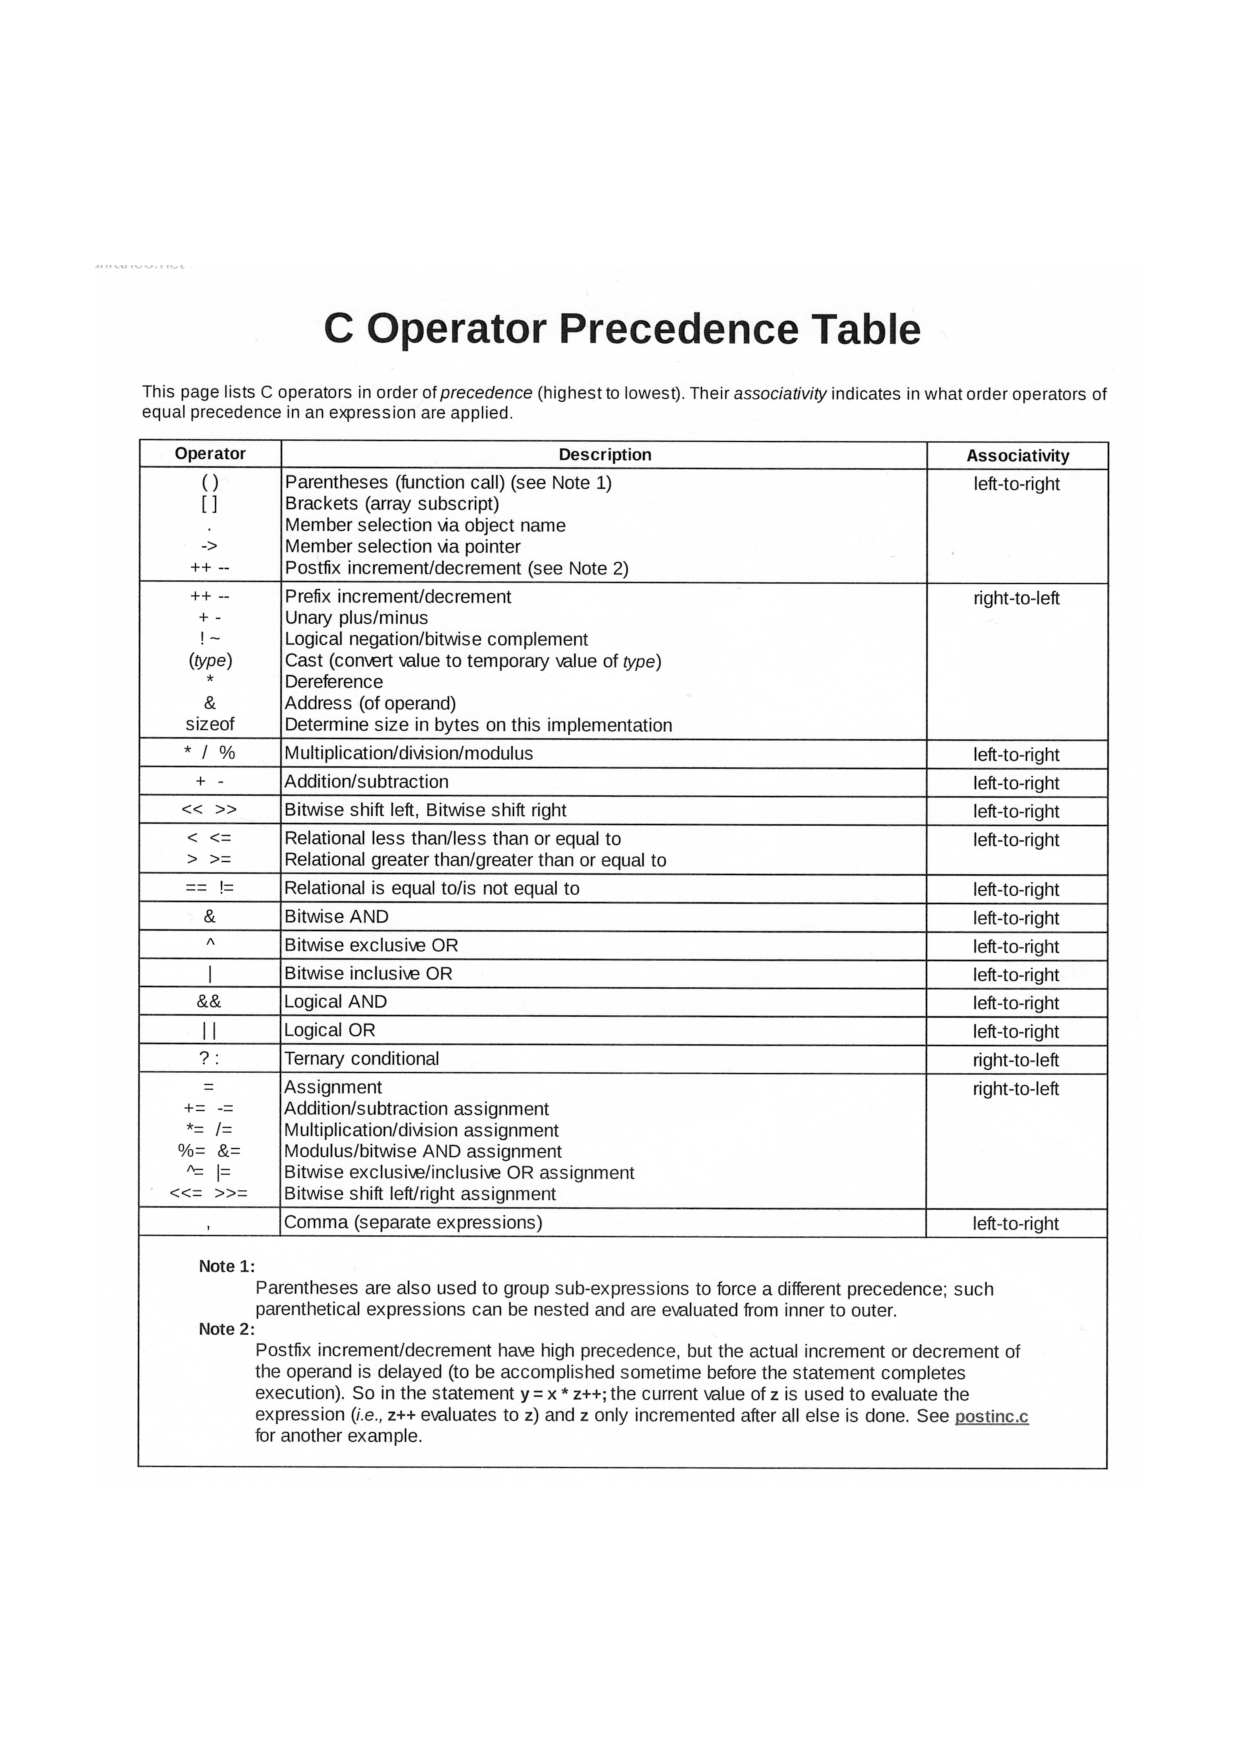
\includepdf[pages={1},landscape=false]{pdf/c_precedence_table.pdf}
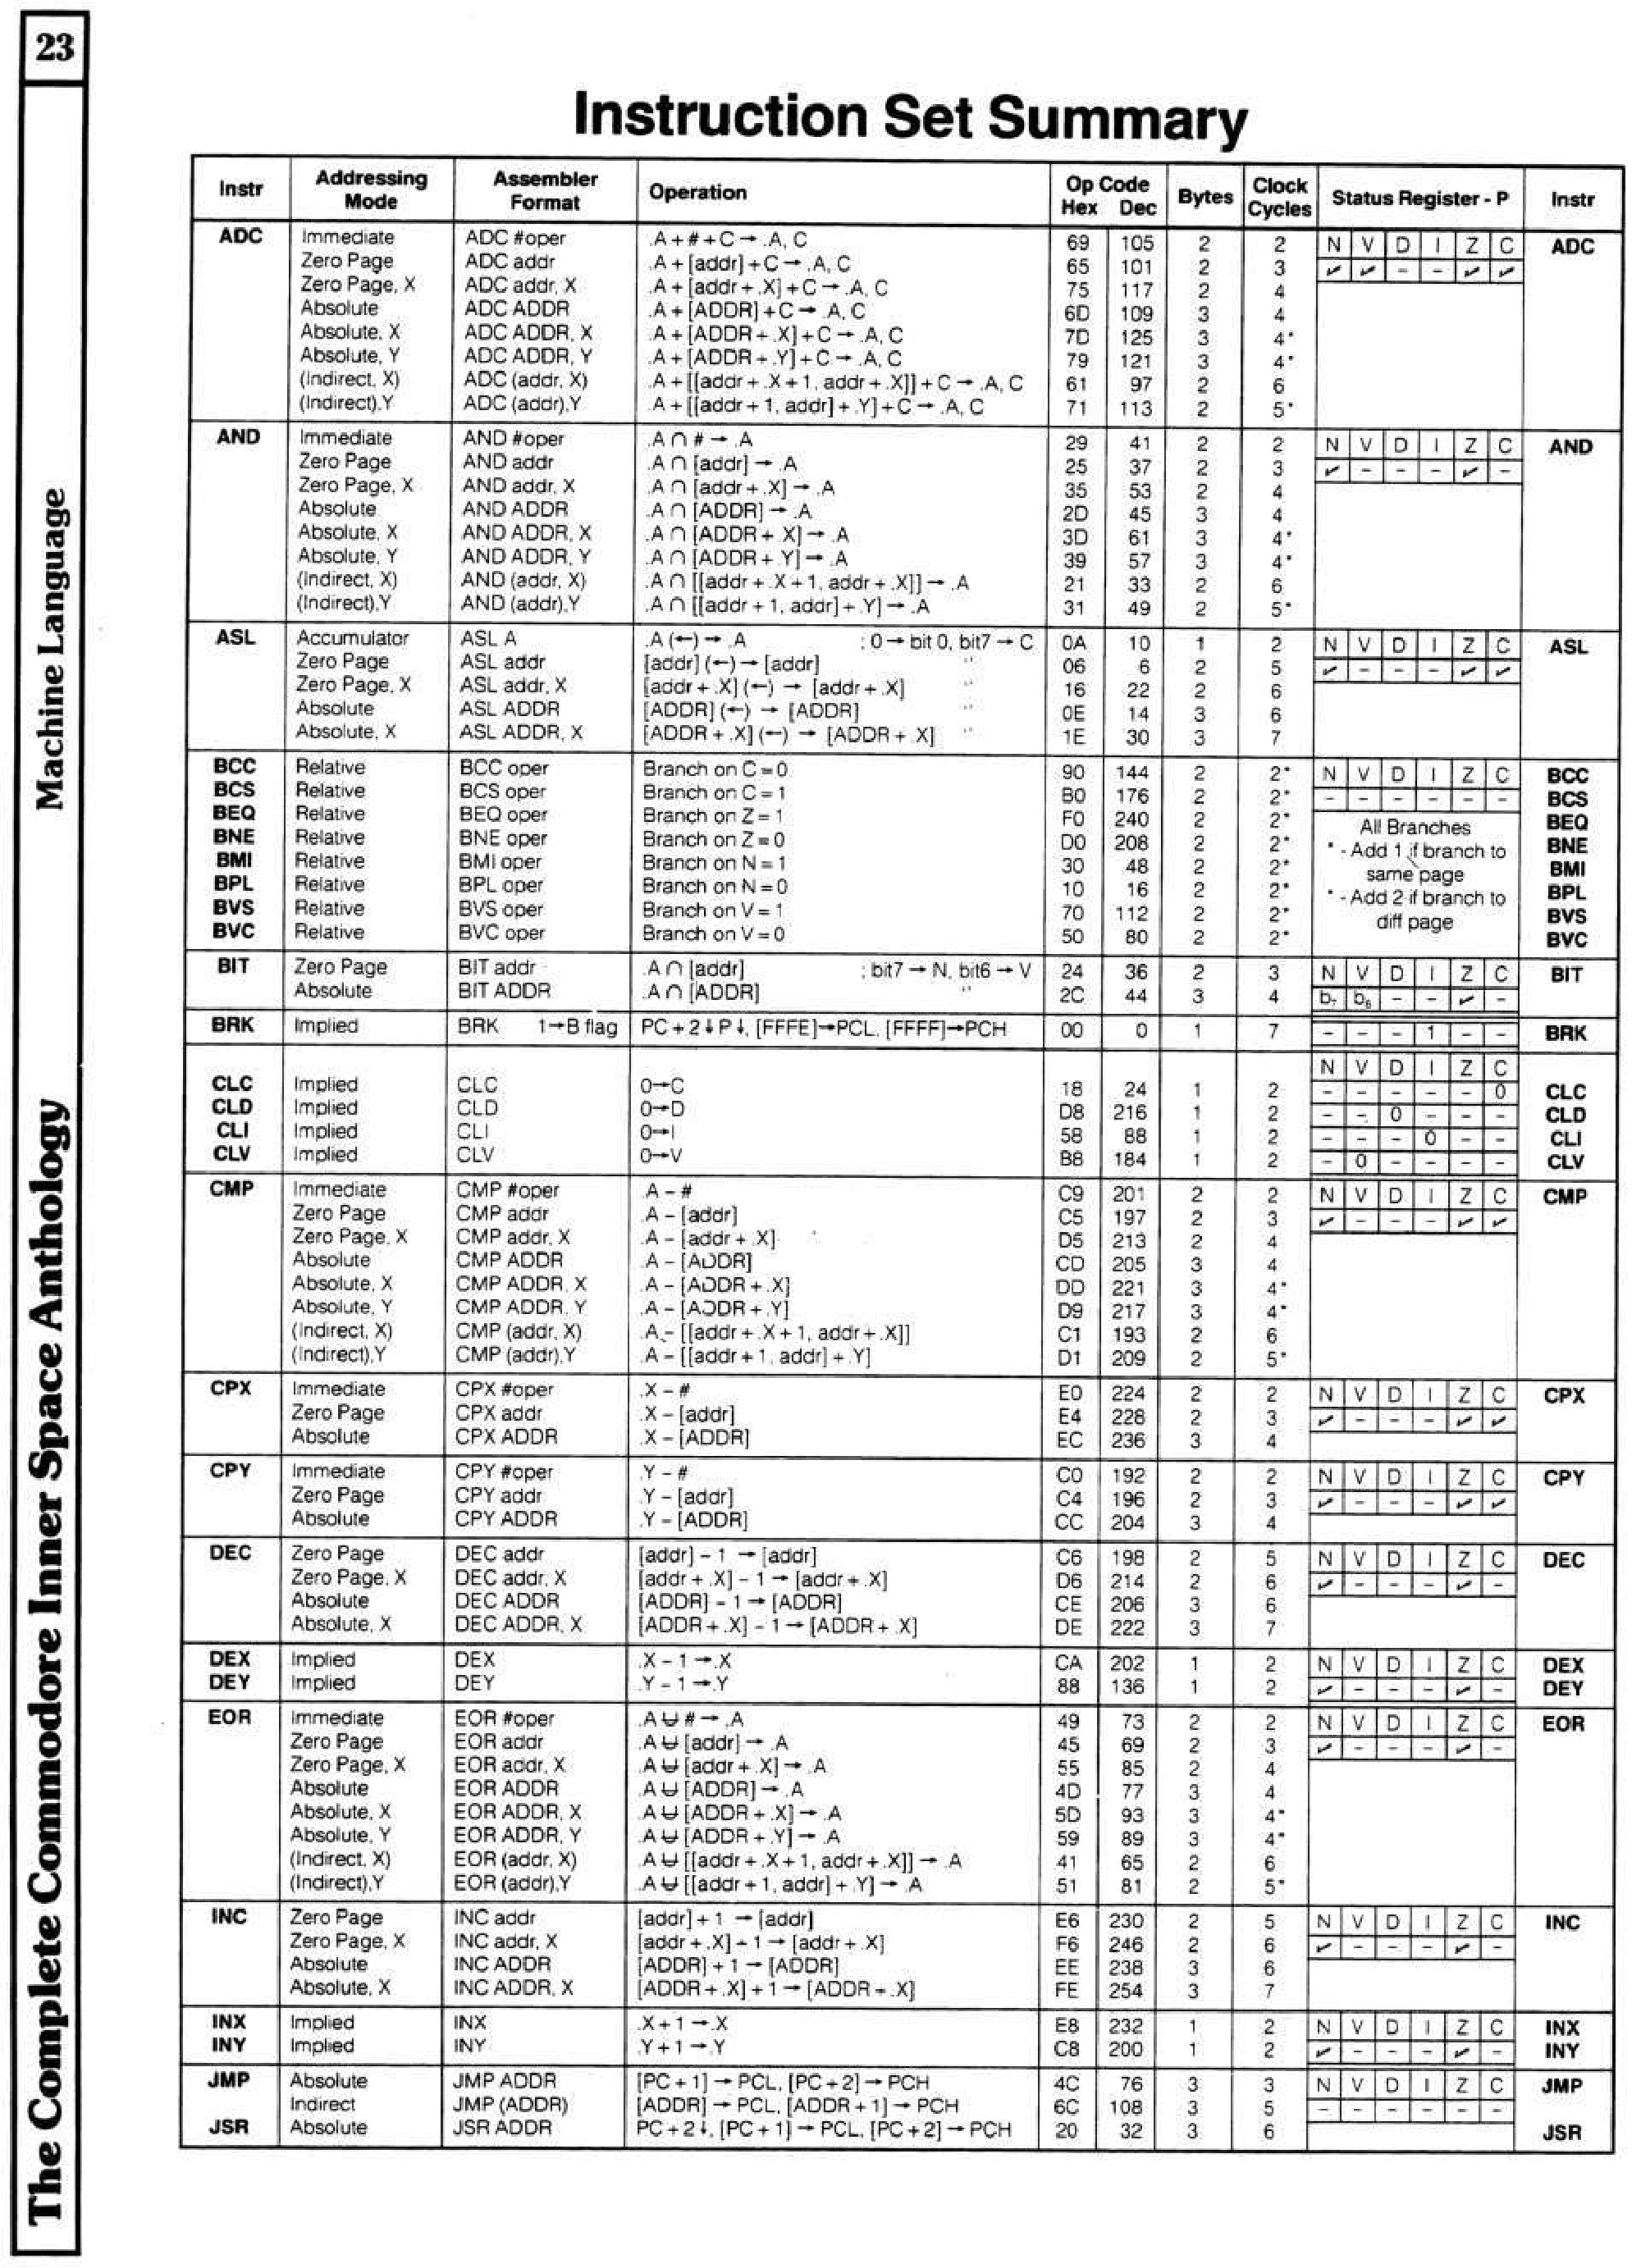
\includepdf[pages={1},landscape=false]{pdf/6502_opcode1.pdf}
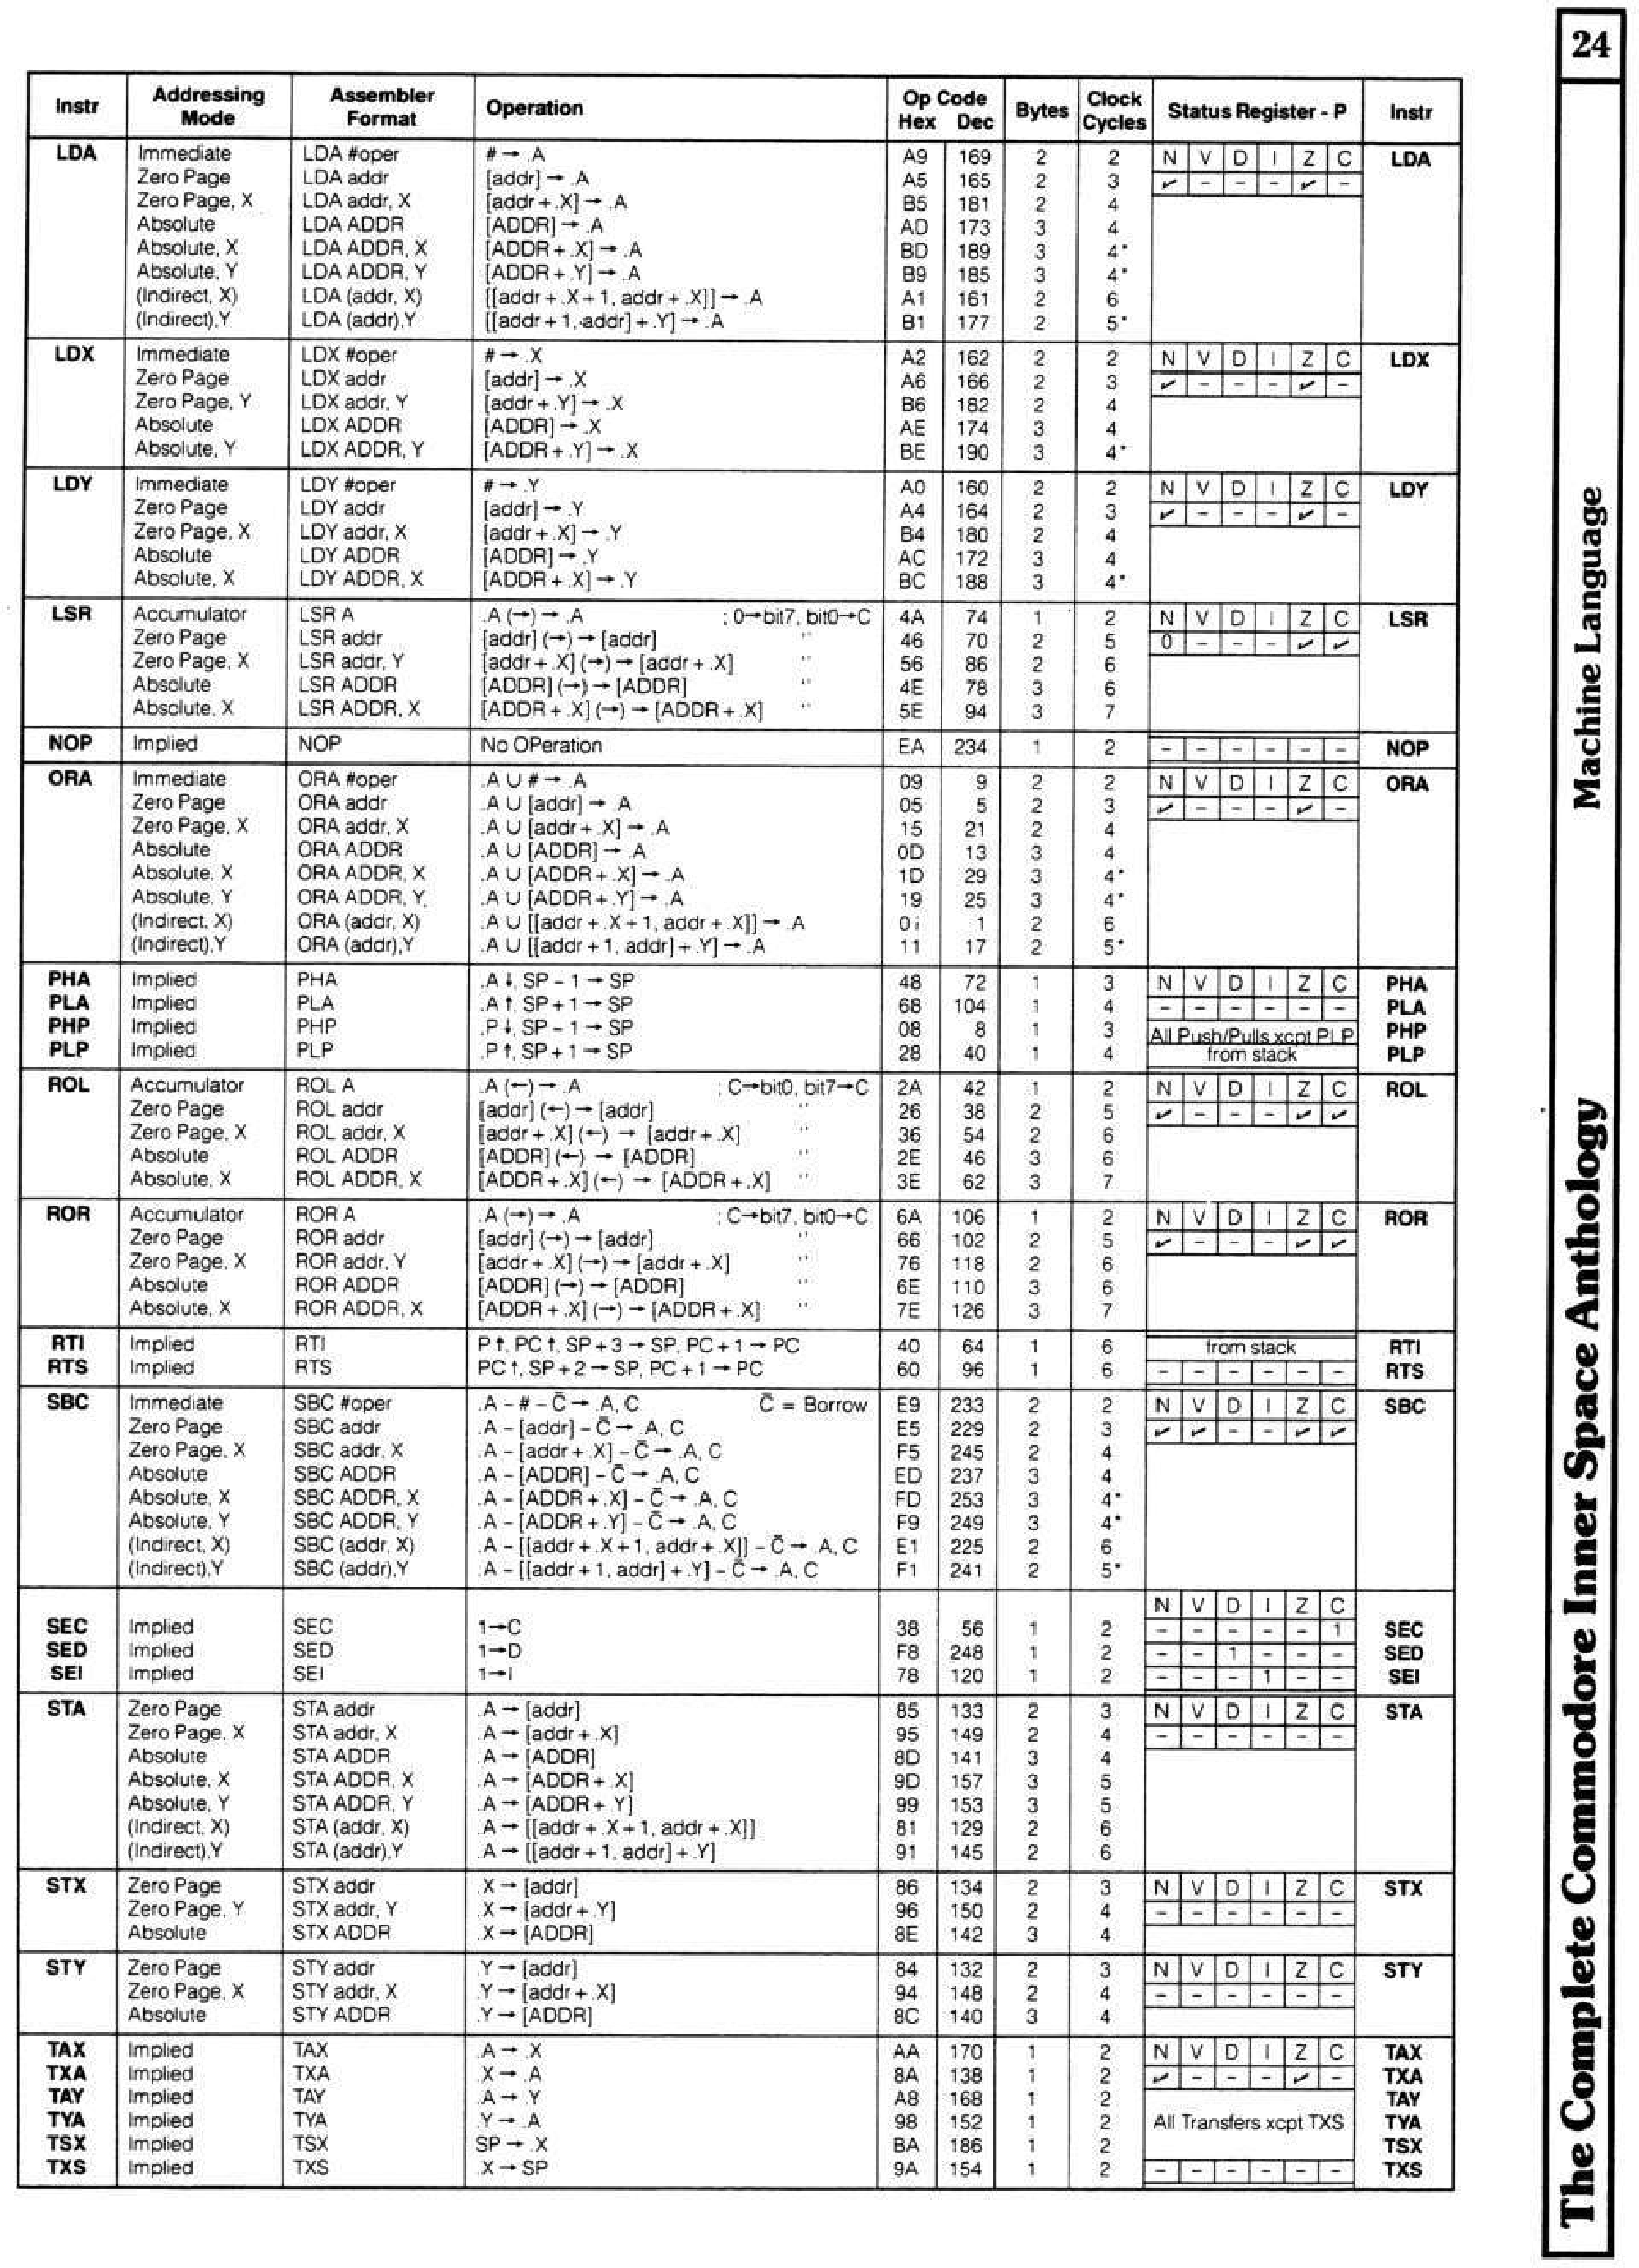
\includepdf[pages={1},landscape=false]{pdf/6502_opcode2.pdf}
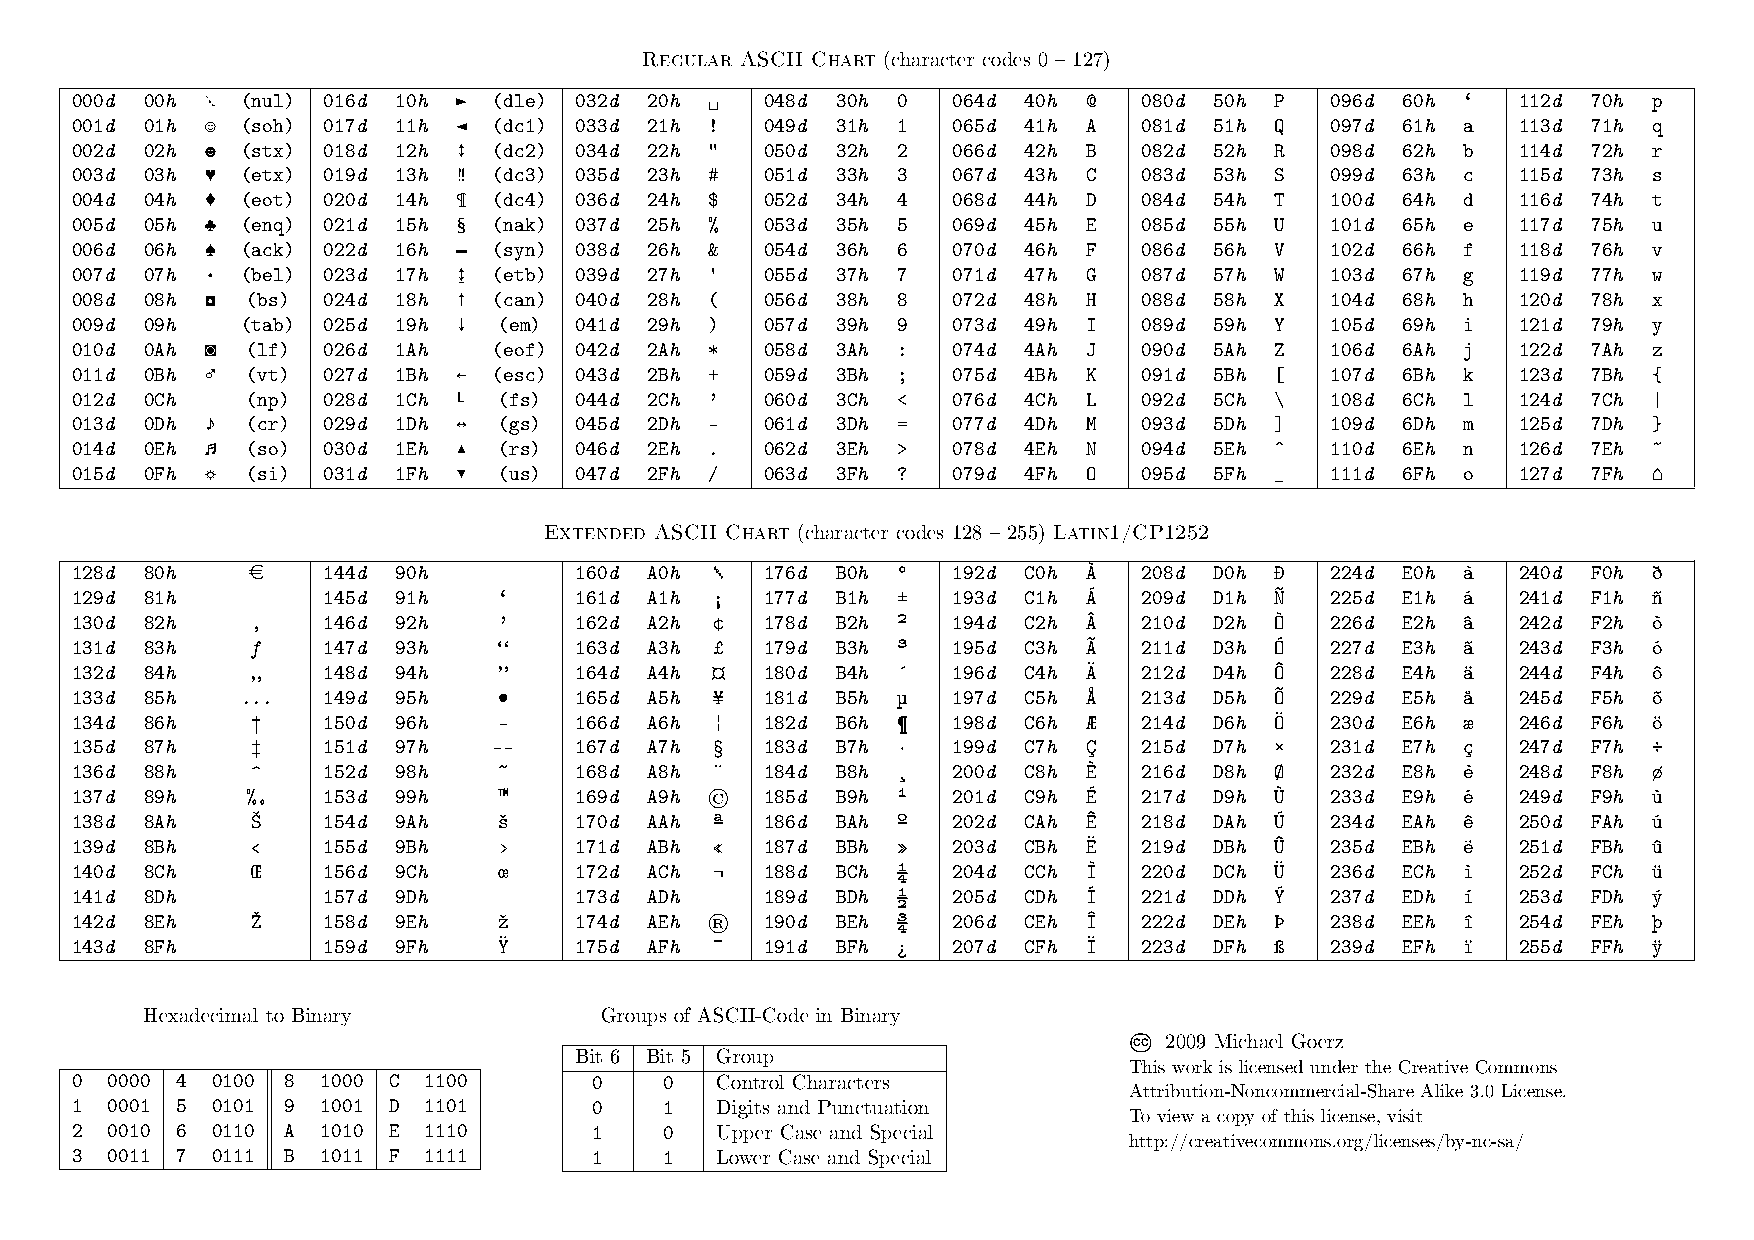
\includepdf[pages={1},landscape=true]{pdf/ascii_table.pdf}

%%%%%%%%%%%%%%%%%%%%%%%%%%%%%%%%%%%%%%%%%%%%%%%%%%%%%%%%%%%%%
%% LITERATUR UND ANDERE VERZEICHNISSE
%%%%%%%%%%%%%%%%%%%%%%%%%%%%%%%%%%%%%%%%%%%%%%%%%%%%%%%%%%%%%
%% Ein kleiner Abstand zu den Kapiteln im Inhaltsverzeichnis (toc)
\addtocontents{toc}{\protect\vspace*{\baselineskip}}


%%%%%%%%%%%%%%%%%%%%%%%%%%%%%%%%%%%%%%%%%%%%%%%%%%%%%%%%%%%%%
%% ANHÄNGE
%%%%%%%%%%%%%%%%%%%%%%%%%%%%%%%%%%%%%%%%%%%%%%%%%%%%%%%%%%%%%
\appendix
%% ==> Schreiben Sie hier Ihren Text oder fügen Sie externe Dateien ein.

%\input{Dateiname} %Eine Datei 'Dateiname.tex' wird hierfür benötigt.


\end{document}

